\documentclass{article}

  % packages
    % basic stuff for rendering math
    \usepackage[letterpaper, top=1in, bottom=1in, left=1in, right=1in]{geometry}
    \usepackage[utf8]{inputenc}
    \usepackage[english]{babel}
    \usepackage{amsmath} 
    \usepackage{amssymb}
    % \usepackage{amsthm}
    \usepackage{bbm}

    % extra math symbols and utilities
    \usepackage{mathtools}        % for extra stuff like \coloneqq
    \usepackage{mathrsfs}         % for extra stuff like \mathsrc{}
    \usepackage{centernot}        % for the centernot arrow 
    \usepackage{bm}               % for better boldsymbol/mathbf 
    \usepackage{enumitem}         % better control over enumerate, itemize
    \usepackage{xr-hyper}
    \usepackage{hyperref}         % for hypertext linking
    \usepackage{fancyvrb}          % for better verbatim environments
    \usepackage{newverbs}         % for texttt{}
    \usepackage{xcolor}           % for colored text 
    \usepackage{listings}         % to include code
    \usepackage{lstautogobble}    % helper package for code
    \usepackage{parcolumns}       % for side by side columns for two column code
    

    % page layout
    \usepackage{fancyhdr}         % for headers and footers 
    \usepackage{lastpage}         % to include last page number in footer 
    \usepackage{parskip}          % for no indentation and space between paragraphs    
    \usepackage[T1]{fontenc}      % to include \textbackslash
    \usepackage{footnote}
    \usepackage{etoolbox}

    % for custom environments
    \usepackage{tcolorbox}        % for better colored boxes in custom environments
    \tcbuselibrary{breakable}     % to allow tcolorboxes to break across pages

    % figures
    \usepackage{pgfplots}
    \pgfplotsset{compat=1.18}
    \usepackage{float}            % for [H] figure placement
    \usepackage{tikz}
    \usepackage{tikz-cd}
    \usetikzlibrary{arrows}
    \usetikzlibrary{positioning}
    \usetikzlibrary{calc}
    \usepackage{graphicx}
    \usepackage{caption} 
    \usepackage{subcaption}

    % for tabular stuff 
    \usepackage{dcolumn}

    \usepackage[nottoc]{tocbibind}
    \pdfsuppresswarningpagegroup=1
    \hfuzz=5.002pt                % ignore overfull hbox badness warnings below this limit

  % New and replaced operators
    \DeclareMathOperator{\Tr}{Tr}
    \DeclareMathOperator{\Sym}{Sym}
    \DeclareMathOperator{\Span}{span}
    \DeclareMathOperator{\std}{std}
    \DeclareMathOperator{\Cov}{Cov}
    \DeclareMathOperator{\Var}{Var}
    \DeclareMathOperator{\Corr}{Corr}
    \DeclareMathOperator{\pos}{pos}
    \DeclareMathOperator*{\argmin}{\arg\!\min}
    \DeclareMathOperator*{\argmax}{\arg\!\max}
    \newcommand{\ket}[1]{\ensuremath{\left|#1\right\rangle}}
    \newcommand{\bra}[1]{\ensuremath{\left\langle#1\right|}}
    \newcommand{\braket}[2]{\langle #1 | #2 \rangle}
    \newcommand{\qed}{\hfill$\blacksquare$}     % I like QED squares to be black

  % Custom Environments
    \tcbset{
      colframe = black,
      colback  = white,
      coltitle = black,
      colbacktitle = black!10,
      breakable, 
      arc=0mm,
      boxrule=1pt,
      left=8pt,
      right=8pt,
      top=6pt,
      bottom=6pt,
      before skip=12pt,
      after skip=12pt,
      bottomrule at break=-1pt,
      toprule at break=-1pt,
      fonttitle=\bfseries,
    }
    \newtcolorbox[auto counter, number within=section]{question}[1][]
    {
      title = \textbf{Question \thetcbcounter ~(#1)}
    }
    \newtcolorbox[auto counter, number within=section]{exercise}[1][]
    {
      title = \textbf{Exercise \thetcbcounter ~(#1)}
    }
    \newtcolorbox[auto counter, number within=section]{solution}[1][]
    {
      title = \textbf{Solution \thetcbcounter}
    }
    \newtcolorbox[auto counter, number within=section]{lemma}[1][]
    {
      title = \textbf{Lemma \thetcbcounter ~(#1)},
    }
    \newtcolorbox[auto counter, number within=section]{theorem}[1][]
    {
      title = \textbf{Theorem \thetcbcounter ~(#1)},
    } 
    \newtcolorbox[auto counter, number within=section]{corollary}[1][]
    {
      title = \textbf{Corollary \thetcbcounter ~(#1)},
    } 
    \newtcolorbox[auto counter, number within=section]{proof}[1][]
    {
      before skip = -7pt,
      before upper = \textit{Proof. },
    } 
    \newtcolorbox[auto counter, number within=section]{definition}[1][]
    {
      title = \textbf{Definition \thetcbcounter ~(#1)}
    }
    \newtcolorbox[auto counter, number within=section]{example}[1][]
    {
      title = \textbf{Example \thetcbcounter ~(#1)}
    } 
    \newtcolorbox[auto counter, number within=section]{code}[1][]
    {
      title = \textbf{Code \thetcbcounter ~(#1)}
    } 

    \definecolor{dkgreen}{rgb}{0,0.6,0}
    \definecolor{gray}{rgb}{0.5,0.5,0.5}
    \definecolor{mauve}{rgb}{0.58,0,0.82}
    \definecolor{lightgray}{gray}{0.93}

    % default options for listings (for code)
    \lstset{
      autogobble,
      frame=ltbr,
      language=C,                           % the language of the code
      aboveskip=3mm,
      belowskip=3mm,
      showstringspaces=false,
      columns=fullflexible,
      keepspaces=true,
      basicstyle={\small\ttfamily},
      numbers=left,
      firstnumber=1,                        % start line number at 1
      numberstyle=\tiny\color{gray},
      keywordstyle=\color{blue},
      commentstyle=\color{dkgreen},
      stringstyle=\color{mauve},
      backgroundcolor=\color{lightgray}, 
      breaklines=true,                      % break lines
      breakatwhitespace=true,
      tabsize=3, 
      xleftmargin=2em, 
      framexleftmargin=1.5em, 
      stepnumber=1
    }

  % Page style
    \pagestyle{fancy}
    \fancyhead[L]{Measure Theory}
    \fancyhead[C]{Muchang Bahng}
    \fancyhead[R]{Fall 2025} 
    \fancyfoot[C]{\thepage / \pageref{LastPage}}
    \renewcommand{\footrulewidth}{0.4pt}          % the footer line should be 0.4pt wide
    \renewcommand{\thispagestyle}[1]{}  % needed to include headers in title page

  % external documents 
   \externaldocument[real-]{../Real_Analysis/paper}[../Real_Analysis/paper.pdf] 

\begin{document}

\title{Measure Theory}
\author{Muchang Bahng}
\date{Fall 2025}

\maketitle
\tableofcontents
\pagebreak

This covers computability theory, complexity theory, and automata theory. 
Alphabet. Boolean logic


\section{Sigma Algebras} 

  In here, we will develop a deeper formalism of set theory and topology, now that we have the tools of analysis. 

\subsection{Set-Theroetic Limits}

  Let's talk about sequences of sets $(A_n)_n$. 

  \begin{definition}[Monotone Sequence]
    A sequence of sets $(A_n)_n$ is called 
    \begin{enumerate}
      \item \textbf{(strictly) increasing} if $A_n \subsetneq A_{n+1}$. 
      \item \textbf{nondecreasing} if $A_n \subseteq A_{n+1}$. 
      \item \textbf{(strictly) decreasing} if $A_n \supsetneq A_{n+1}$. 
      \item \textbf{nonincreasing} if $A_n \supseteq A_{n+1}$. 
    \end{enumerate}
  \end{definition}

  \begin{definition}[Limsup and Liminf of Sets]
    Given a sequence of sets $(A_n)_n$, the \textbf{limsup} and \textbf{liminf} of them can be defined in the equivalent ways. 
    \begin{enumerate}
      \item The \textbf{liminf} is the set of points that are missing in only a finite number of sets, and the \textbf{limsup} is the set of points that are in an infinite number of sets. 
      \begin{align}
        \liminf_{n \to \infty} A_n & \coloneqq \bigcup_{n=1}^\infty \bigcap_{m=n}^\infty A_m \\
        \limsup_{n \to \infty} A_n & \coloneqq \bigcap_{n=1}^\infty \bigcup_{m=n}^\infty A_m 
      \end{align} 

      \item The \textbf{liminf} and \textbf{limsup} are the set of points $x$ where the liminf and limsup of the indicator function function evaluated at $x$ equals $1$. 
        \begin{align}
          \liminf_{n \to \infty} A_n & \coloneqq \{x \in X \mid \liminf_{n \to \infty} \mathbbm{1}_{A_n} (x) = 1 \} \\ 
          \limsup_{n \to \infty} A_n & \coloneqq \{x \in X \mid \limsup_{n \to \infty} \mathbbm{1}_{A_n} (x) = 1 \}
        \end{align}

    \end{enumerate}
    Both liminf and limsup always exist for any sequence of sets. 
  \end{definition} 
  \begin{proof}
    DeMorgan's law. 
  \end{proof}

  \begin{lemma}[Monotonicity]
    For any sequence of sets 
    \begin{equation}
      \liminf_{n \to \infty} A_n \subseteq \limsup_{n \to \infty} A_n 
    \end{equation}
  \end{lemma}

  \begin{lemma}[Complements]
    \begin{equation}
      \liminf_{n \to \infty} A_n = \bigg( \limsup_{n \to \infty} A_n^c  \bigg)^c
    \end{equation}
  \end{lemma}
  \begin{proof}
    
  \end{proof}

  \begin{definition}[Limit of Sets]
    
  \end{definition} 

\subsection{Borel Hierarchy}

  \begin{definition}[$F_\sigma$ Sets]
    A \textbf{$F_\sigma$-set} is a subset of a topological space that is a countable union of closed sets. 
  \end{definition}

  \begin{definition}[$G_\delta$ Sets]
    A \textbf{$G_\delta$-set} is a subset of a topological space  that is a countable intersection of open sets. 
  \end{definition}

  \begin{lemma}
    The complement of a $F_\sigma$ set is a $G_\delta$ set. 
  \end{lemma} 

\subsection{Sigma Algebra}

  Now, given any set $X$, we can construct its power set $2^X$. But we can't naively just give a measure to every $A \in 2^X$, since for certain spaces, this causes nasty contradictions shown through the Banach-Tarski Paradox.\footnote{Given any two bounded subsets $A$ and $B$ of $\mathbb{R}^n$ where $n \geq 3$, both of which have a nonempty interior, there are partitions of $A$ and $B$ into a finite number of disjoint subsets, $A = A_1 \cup \ldots \cup A_k$, $B = B_1 \cup \ldots \cup B_k$, such that $A_i$ and $B_i$ are congruent for every $i \in [k]$.} A nice set of subsets of $X$ to work with is the $\sigma$-algebra of $X$. 

  \begin{definition}[$\sigma$-Algebra]
    A \textbf{$\boldsymbol{\sigma}$-algebra} on a set $X$ is a collection  of subsets of $X$, denoted $\mathcal{A} \subset 2^X$ that contains $\emptyset$, $X$ itself, is stable under a countable union, and is stable under complementation. This pair $(X, \mathcal{A})$ is called a \textbf{measurable space}. 
  \end{definition}

  \begin{lemma}[Additional Property of $\sigma$-Algebras]
    A commonly known property of any $\sigma$-algebra $\mathcal{A}$ is that it is stable under countable intersections, too. 
    \begin{equation}
      A_1, A_2, \ldots, \in \mathcal{A} \implies \bigcap_{k=1}^\infty A_k \in \mathcal{A}
    \end{equation}
  \end{lemma}
  \begin{proof}
    We can utilize the fact that 
    \begin{equation}
      \bigcap_{k=1}^\infty A_k = X \setminus \bigcup_{k=1}^\infty A_k^c
    \end{equation}
  \end{proof}

  A $\sigma$-algebra is similar to the topology $\tau$ of topological space. Both $\mathcal{A}$ and $\tau$ require $\emptyset$ and $X$ to be in it. The three differences are that (i) $\tau$ does not allow compelmentation, (ii) $\tau$ allows any (even uncountable) union of sets (condition is strengthened), and (iii) $\tau$ allows only finite intersection of sets (condition is weakened). Now in order to construct $\sigma$-algebras, the following theorems are useful since they allow us to construct $\sigma$-algebras from other $\sigma$-algebras. It turns out that the intersection of $\sigma$-algebras is a $\sigma$-algebra, but not for unions. 

  \begin{theorem}[Intersection of Sigma Algebras is a Sigma Algebra]
    Let $\{\mathcal{A}_k\}$ be a family of $\sigma$-algebras of $X$. Then, $\cap \mathcal{A}_k$ is also a $\sigma$-algebra of $X$. 
  \end{theorem}
  \begin{proof}
    Clearly, $\emptyset, X$ is in $\cap \mathcal{A}_k$. To prove complementation, 
    \begin{equation}
      A \in \bigcap \mathcal{A}_k \implies A \in \mathcal{A}_k \; \forall k \implies A^c \in A_k \; \forall k \implies A^c \in \bigcap \mathcal{A}_k
    \end{equation}
    To prove countable union, let $\{A_j\}_{j \in J}$ be some countable family of subsets in $\cap \mathcal{A}_k$. Then, 
    \begin{equation}
      A_j \in \bigcap \mathcal{A}_k \; \forall j \in J \implies A_j \in \mathcal{A}_k \; \forall k \forall j \implies \bigcup A_j \in \mathcal{A}_k \; \forall k \implies \bigcup A_j \in \bigcap \mathcal{A}_k
    \end{equation}
  \end{proof}

  This allows us to easily prove the following theorem, which just establishes the existence of $\sigma$-algebras. 

  \begin{theorem}[Unique Smallest Sigma Algebra]
    Let $F \subset 2^X$. Then there exists a unique smallest $\sigma$-algebra $\sigma(F)$ containing $F$, called the $\sigma$-algebra \textbf{generated} by $F$. 
  \end{theorem}
  \begin{proof}
    Let us denote $\mathcal{M}$ as the set of all possible $\sigma$-algebras $\mathcal{B}$ of $X$. $\mathcal{M}$ is nonempty since it contains $2^X$. Then, the intersection 
    \begin{equation}
      \bigcap_{\mathcal{B} \in \mathcal{M}} \mathcal{B}
    \end{equation}
    is the unique smallest $\sigma$-algebra. 
  \end{proof} 

  With this guarantee, we can now define what it means for a set of subsets to \textit{generate} a $\sigma$-algebra. 

  \begin{definition}[$\sigma$-Algebra Generated by a Set]
    Given a collection of sets $\mathscr{C}$, the $\sigma$-algebra \textbf{generated} by $\mathscr{C}$ is the unique smallest $\sigma$-algebra containing $\mathscr{C}$, denoted $\sigma(\mathscr{C})$. 
  \end{definition} 

  This gives us a convenient way to construct $\sigma$-algebras. The general method is to identify a collection of ``important'' subsets that we would like to be included in the $\sigma$-algebra, and then just generate it.   

  \begin{definition}[Borel $\sigma$-algebra]
    The \textbf{Borel $\boldsymbol{\sigma}$-algebra} of a topological space $(X, \mathscr{T})$ is the $\sigma$-algebra generated by the topology $\mathscr{T}$, denoted $\mathcal{B}(X) \coloneqq \sigma(\mathscr{T})$. An element of the Borel algebra is called a \textbf{Borel set}. 
  \end{definition}

  Note that the Borel algebra contains: 
  \begin{enumerate}
    \item all open sets, 
    \item all closed sets due to closure under complements, 
    \item all $G_\delta$ sets due to closure under countable unions, 
    \item all $F_\sigma$ sets due to closure under countable intersection. 
  \end{enumerate}

  \begin{definition}[Measure Space]
    A \textbf{measure set} is a tuple $(X, \mathcal{A})$, where $X$ is an arbitrary space and $\mathcal{A}$ a $\sigma$-algebra. 
  \end{definition}

\section{Measures and Sigma Algebras}

  Now, given any set $X$, we can construct its power set $2^X$. But we can't naively just give a measure to every $A \in 2^X$, since for certain spaces, this causes nasty contradictions shown through the Banach-Tarski Paradox. 

  \begin{theorem}[Banach-Tarski Paradox (Strong Form)]
    Given any two bounded subsets $A$ and $B$ of $\mathbb{R}^n$ where $n \geq 3$, both of which have a nonempty interior, there are partitions of $A$ and $B$ into a finite number of disjoint subsets, $A = A_1 \cup \ldots \cup A_k$, $B = B_1 \cup \ldots \cup B_k$, such that $A_i$ and $B_i$ are congruent for every $i \in [k]$. 
  \end{theorem}

  A nice set of subsets of $X$ to work with is the $\sigma$-algebra of $X$. 

  \begin{definition}[$\sigma$-Algebra]
    A \textbf{$\boldsymbol{\sigma}$-algebra} on a set $X$ is a collection  of subsets of $X$, denoted $\mathcal{A} \subset 2^X$ that contains $\emptyset$, $X$ itself, is stable under a countable union, and is stable under complementation. This pair $(X, \mathcal{A})$ is called a \textbf{measurable space}. 
  \end{definition}

  \begin{lemma}[Additional Property of $\sigma$-Algebras]
    A commonly known property of any $\sigma$-algebra $\mathcal{A}$ is that it is stable under countable intersections, too. 
    \begin{equation}
      A_1, A_2, \ldots, \in \mathcal{A} \implies \bigcap_{k=1}^\infty A_k \in \mathcal{A}
    \end{equation}
  \end{lemma}
  \begin{proof}
    We can utilize the fact that 
    \begin{equation}
      \bigcap_{k=1}^\infty A_k = X \setminus \bigcup_{k=1}^\infty A_k^c
    \end{equation}
  \end{proof}

  A $\sigma$-algebra is similar to the topology $\tau$ of topological space. Both $\mathcal{A}$ and $\tau$ require $\emptyset$ and $X$ to be in it. The three differences are that (i) $\tau$ does not allow compelmentation, (ii) $\tau$ allows any (even uncountable) union of sets (condition is strengthened), and (iii) $\tau$ allows only finite intersection of sets (condition is weakened). Now in order to construct $\sigma$-algebras, the following theorems are useful since they allow us to construct $\sigma$-algebras from other $\sigma$-algebras. It turns out that the intersection of $\sigma$-algebras is a $\sigma$-algebra, but not for unions. 

  \begin{theorem}[Intersection of Sigma Algebras is a Sigma Algebra]
    Let $\{\mathcal{A}_k\}$ be a family of $\sigma$-algebras of $X$. Then, $\cap \mathcal{A}_k$ is also a $\sigma$-algebra of $X$. 
  \end{theorem}
  \begin{proof}
    Clearly, $\emptyset, X$ is in $\cap \mathcal{A}_k$. To prove complementation, 
    \begin{equation}
      A \in \bigcap \mathcal{A}_k \implies A \in \mathcal{A}_k \; \forall k \implies A^c \in A_k \; \forall k \implies A^c \in \bigcap \mathcal{A}_k
    \end{equation}
    To prove countable union, let $\{A_j\}_{j \in J}$ be some countable family of subsets in $\cap \mathcal{A}_k$. Then, 
    \begin{equation}
      A_j \in \bigcap \mathcal{A}_k \; \forall j \in J \implies A_j \in \mathcal{A}_k \; \forall k \forall j \implies \bigcup A_j \in \mathcal{A}_k \; \forall k \implies \bigcup A_j \in \bigcap \mathcal{A}_k
    \end{equation}
  \end{proof}

  This allows us to easily prove the following proposition, which just establishes the existence of $\sigma$-algebras. 

  \begin{proposition}[Unique Smallest Sigma Algebra]
    Let $F \subset 2^X$. Then there exists a unique smallest $\sigma$-algebra $\sigma(F)$ containing $F$, called the $\sigma$-algebra \textbf{generated} by $F$. 
  \end{proposition}
  \begin{proof}
    Let us denote $\mathcal{M}$ as the set of all possible $\sigma$-algebras $\mathcal{B}$ of $X$. $\mathcal{M}$ is nonempty since it contains $2^X$. Then, the intersection 
    \begin{equation}
      \bigcap_{\mathcal{B} \in \mathcal{M}} \mathcal{B}
    \end{equation}
    is the unique smallest $\sigma$-algebra. 
  \end{proof}

  Now, we can introduce the first nontrivial $\sigma$-algebra, called the Borel $\sigma$-algebra. 

  \begin{definition}[Borel $\sigma$-algebra]
    The \textbf{Borel $\boldsymbol{\sigma}$-algebra} of a topological space $(X, \mathscr{T})$ is the $\sigma$-algebra generated by the topology $\mathscr{T}$, denoted $\mathcal{B}(X) \coloneqq \sigma(\mathscr{T})$. 
  \end{definition} 

  \begin{definition}[Limsup and Liminf of Sets]
    Given a collection of sets $(A_n)_n$, we can define the limsup and liminf of a sequence of them. 
    \begin{enumerate}
      \item All points that are missing in only a finite number of sets. 
        \begin{equation}
          \liminf A_n \coloneqq \bigcup_{n=1}^\infty \bigcap_{m=n}^\infty A_m 
        \end{equation}

      \item All points that are in an infinite number of sets 
        \begin{equation}
          \limsup A_n = \bigcap_{n=1}^\infty \bigcup_{m=n}^\infty A_m 
        \end{equation}
    \end{enumerate}
  \end{definition}

  Now, how do we measure a size on $\mathcal{B}(X)$? We use measures. 

  \begin{definition}[Measure]
    Given a measurable space $(X, \mathcal{A})$, a \textbf{measure} is a function $\mu : \mathcal{A} \longrightarrow [0, +\infty]$ satisfying 
    \begin{enumerate}
      \item Null empty set $\mu(\emptyset) = 0$ 
      \item Countable additivity: For all countable collections $\{A_k\}_{k=1}^\infty$ of pairwise disjoint subsets $A_k \in \mathcal{A}$, 
      \begin{equation}
        \mu \bigg( \bigsqcup_{k=1}^\infty A_k \bigg) = \sum_{k=1}^\infty \mu(A_k)
      \end{equation}
      Remember that we are allowed to take countable unions inside our $\sigma$-algebra, so this makes sense. 
    \end{enumerate}
    This immediately implies that given $A, B \in \mathcal{A}$, then $A \subset B \implies \mu(A) \leq \mu(B)$. The triplet $(X, \mathcal{A}, \mu)$ is called a \textbf{measure space}. 
  \end{definition}

  The first condition is important because it allows us to take finite disjoint unions. That is, since $\mu(A_1 \cup A_2) = \mu(A_1 \cup A_2 \cup \emptyset \cup \ldots)$, we have 
  \begin{equation}
    \sum_{k=1}^\infty = \mu(A_1) + \mu(A_2)
  \end{equation}
  Disjointness is clearly important since if it wasn't, then $\mu(A) = \mu(A \cup A) = 2 \mu(A)$, which is absurd. Now our natural measure on the real number line with its Borel $\sigma$-algebra $(\mathbb{R}, \mathcal{B})$, we want a measure satisfying $\mu((a, b)) = b - a$ and $\mu([0, \infty)) = \infty$. Such a measure does exist, and it is called the Lebesgue measure, but proving its existence is highly nontrivial. Let us first look into some properties of measures, which all seem natural. 

  \begin{proposition}
    If $A_1 \subset A_2 \subset A_3 \subset \ldots$, then 
    \begin{equation}
      \mu\bigg( \bigcup_{k=1}^\infty A_k \bigg) = \lim_{k \rightarrow \infty} \mu(A_k)
    \end{equation}
  \end{proposition}
  \begin{proof}
    This is the first time we introduce limits. With the fact that $\mu(A_k)$ must be nondecreasing, we can use real analysis and see that it is bounded by $\infty$, meaning that it must have a limit. But why does this limit equal to the left hand side? We can see that 
    \begin{align}
      \mu\bigg( \bigcup_{k=1}^\infty A_k \bigg) & = \mu(A_1) + \sum_{k=2}^\infty \mu(B_k) \\
      & = \mu(A_1) + \lim_{k \rightarrow \infty} \sum_{k=2}^\infty \mu(B_k) \\
      & = \lim_{k \rightarrow \infty} \mu(A_1 \cup B_2 \cup \ldots B_k)  = \lim_{k \rightarrow \infty} \mu(A_k) 
    \end{align}
    where $B_k = A_k \setminus A_{k-1}$. 
  \end{proof}

  Now a similar theorem, but with a little twist to it. 

  \begin{proposition}
    If $A_1 \supset A_2 \supset A_3 \supset \ldots$, then 
    \begin{equation}
      \mu\bigg( \bigcap_{k=1}^\infty A_k \bigg) = \lim_{k \rightarrow \infty} \mu(A_k)
    \end{equation}
    if $\mu(A_1) < \infty$. 
  \end{proposition}
  \begin{proof}
    The $\mu(A_1) < \infty$ is a necessary condition, since if we take $A_k = [k, \infty)$ on the real number line, then we have $\cap_{k=1}^\infty A_k = \emptyset$, but the limit of the measure is $\infty$. Well we can define $B_k = A_k \setminus A_{k+1}$ and write $\cap_{k=1}^\infty A_k = A_1 \setminus \cup_{k=1}^\infty B_k$, which means that 
    \begin{align*}
      \mu\bigg( \bigcap_{k=1}^\infty A_k \bigg) & = \mu\bigg( A_1 \setminus \bigcup_{k=1}^\infty B_k \bigg) \\
      & = \mu(A_1) - \mu\bigg( \bigcup_{k=1}^\infty B_k\bigg) \\
      & = \mu(A_1) - \sum_{k=1}^\infty \mu(B_k) \\
      & = \mu(A_1) - \lim_{K \rightarrow \infty} \sum_{k=1}^K \mu(B_k) \\
      & = \lim_{K \rightarrow \infty} \bigg( \mu(A_1) - \sum_{k=1}^K \mu(B_k) \bigg) \\
      & = \lim_{K \rightarrow \infty} \mu \bigg( A_1 \setminus \bigcup_{k=1}^K B_k \bigg) = \lim_{K \rightarrow \infty} \mu(A_K)
    \end{align*}
    Now the first line uses the fact that if $A \subset B$, then $\mu(B \setminus A) + \mu(A) = \mu(B)$, and with the further assumption that $\mu(A) < \infty$, we can subtract on both sides like we do with regular arithmetic. 
  \end{proof}

\subsection{Outer Measures, Construction of Lebesgue Measure}

  Now let's try to construct a measure $\lambda$ on the Borel $\sigma$-algebra $\mathcal{B}(\mathbb{R})$ that assigns length, i.e. $\lambda([a, b]) = b - a$. We will do so by constructing outer measures $\lambda^*: 2^\mathbb{R} \longrightarrow \mathbb{R}$ that acts on the power set of $\mathbb{R}$ s.t. $\lambda^*([a, b]) = b - a$. But this turns out to have its own problems and contradictions, so once we construct such a $\lambda^*$, we will "throw away" all the sets that don't behave nicely under $\lambda^*$ and just use its restriction on the Borel algebra. It turns out that the sets that do behave well under $\lambda^*$ is bigger than the Borel algebra, call it $\mathcal{M}_{\lambda^*}$. So, we have $\mathcal{B}(\mathbb{R}) \subset \mathcal{M}_{\lambda^*} \subset 2^\mathbb{R}$. We will do this in full generality in the following way. We take any space $X$ and construct an outer measure $\mu^*$ on its power set $2^X$. Then, we construct the $\sigma$-algebra of well-behaved sets $\mathcal{M}_{\mu^*} \subset 2^X$, and define our measure $\mu$ on $\mathcal{M}_{\mu^*}$. When defining our outer measure, the condition that the outer measure of a disjoint union of subsets is equal to the sum of the outer measure of the subsets is a bit too restricting, so we use a softer condition. 

  \begin{definition}[Outer Measure]
    A function $\mu^* : 2^X \longrightarrow [0, \infty]$ is an \textbf{outer measure} if $\mu^*(\emptyset) = 0$, $A \subset B \implies \mu^* (A) \leq \mu^*(B)$, and 
    \begin{equation}
      \mu^* \bigg( \bigcup_{k=1}^\infty A_k \bigg) \leq \sum_{k=1}^\infty \mu^* (A_k)
    \end{equation}
    This final condition removes the fact that they must be disjoint, and now we have an inequality. 
  \end{definition}

  Now to construct our Lebesgue outer measure, let us define the following on $\mathbb{R}$. It's a hard definition, but a natural one, since we're taking all these intervals and trying to make them as snug as possible to define the outer measure of an arbitrary set. 

  \begin{definition}[Lebesgue Outer Measure of $\mathbb{R}$]
    Given $A \subset \mathbb{R}$, let 
    \begin{equation}
      C_A = \big\{ \{(a_j, b_j)\}_{j=1}^\infty \mid A \subset \bigcup_{j=1}^\infty (a_j, b_j) \big\}
    \end{equation}
    This is more complicated than it looks. Given a set $A$, we are looking at a family of all collections of intervals that cover $A$. Clearly, all coverings in $C_A$ must have a length greater than $A$, and their length can be easily measured by summing up the intervals $\sum_{j=1}^\infty (b_j - a_j)$. So, we can define the outer measure of $A$ to be the infimum of these sums. 
    \begin{equation}
      \lambda^*(A) = \inf_{C_A} \sum_{j=1}^\infty (b_j - a_j)
    \end{equation}
    We can also generalize this further by introducing a increasing, continuous function $F: \mathbb{R} \rightarrow \mathbb{R}$ and defining the outer measure to be 
    \begin{equation}
     \lambda^*(A) = \inf_{C_A} \sum_{j=1}^\infty \big( F(b_j) - F(a_j) \big) 
    \end{equation}
  \end{definition}

  \begin{example}[Rationals have Outer Measure $0$]
    Let us prove that $\lambda^*(\mathbb{Q}) = 0$. It is countable so we can enumerate it $\mathbb{Q} = \{ q_j\}_{j=1}^\infty$. This is counterintuitive, because since $\mathbb{Q}$ is dense in $\mathbb{R}$, in order to make a covering of $\mathbb{Q}$ we sort of have to cover the entire real line. Visually, this is hard, but it is pretty simple to show that you don't have to. We pick $\epsilon > 0$ and define 
    \begin{equation}
      I_j = \big( q_j - \frac{\epsilon}{2^j} , q_j + \frac{\epsilon}{2^j} \big)
    \end{equation}
    So, 
    \begin{equation}
      \sum_{j=1}^\infty |I_j| = \sum_{j=1}^\infty \frac{\epsilon}{2^j} = 2 \epsilon
    \end{equation}
    This collection $\{I_j\}$ is one element of $C_\mathbb{Q}$ of coverings of the rationals, and taking $\epsilon$ as small as we want, the infimum is $0$. This can be done with all countable subsets of $\mathbb{R}$. 
  \end{example}

  \begin{definition}[Almost Everywhere]
    Given a measure space $(X, \mathcal{A}, \mu)$, a subset $A \in \mathcal{A}$ is said to be a $\mu$-null set if $\mu(A) = 0$. If some property holds for all points $x \in X$ except on a null set, then we say that the property holds \textbf{almost everywhere}.
  \end{definition}

  \begin{example}[Rational Function]
    The function $f(x) = \frac{1}{\sqrt{|x|}}$ is less than $\infty$ almost everywhere. 
  \end{example}

  \begin{proposition}[$\lambda^*$ is an Outer Measure]
    The first condition is trivial. As for 2, if I have $A \subset B \subset \mathbb{R}$ and have a covering of $B$, then I also have a covering of $A$, and so the infimum corresponding to the covering of $B$ must be greater than or equal to the infimum of that corresponding to the covering of $A$. For 3, we want to prove that the outer measure of the union of $A_k$'s is less than or equal to the sum of the outer measures of the $A_k$'s. We pick $\epsilon > 0$ and have some covering $\{(a^k_j, b^k_j)\}_{j=1}^\infty \in C_{A^k}$. So we have 
    \begin{equation}
      \lambda^*(A_k) \leq \sum_{j=1}^\infty b^k_j - a^k_j
    \end{equation}
    We want the inequality to go the other way around, but we can't do that. But note that $\lambda^* (A_k)$ is the infimum of all coverings $\{(a^k_j, b^k_j)\}_{j=1}^\infty$ of $A_k$, and so we can choose a covering that is as close to $\lambda^* (A_k)$, and then add a term of $\epsilon$ to $\lambda^*(A_k)$ to make it greater than this covering. This is an important step of the proof that is used often! 
    \begin{equation}
      \frac{\epsilon}{2^k} + \lambda^* (A_k) \geq \sum_{j=1}^\infty b_j^k - a_j^k 
    \end{equation}
    Now, 
    \begin{equation}
      A = \bigcup_{k=1}^\infty A_k \subset \bigcup_{k=1}^\infty \bigcup_{j=1}^\infty (a_j^k, b_j^k)
    \end{equation}
    and we can see that $\{(a_j^k , b_j^k)\}_{j, k=1}^\infty \in C_A$ is a countable covering of $A$ (since the countable union of a countable union is countable), implying that 
    \begin{equation}
      \lambda^* (A) \leq \sum_{k=1}^\infty \sum_{j=1}^\infty (b_j^k - a_j^k) \leq \sum_{k=1}^\infty \bigg( \lambda^* (A_k) + \frac{\epsilon}{2^k} \bigg) = \epsilon + \sum_{k=1}^\infty \lambda^*(A_k)
    \end{equation}
    and so setting $\epsilon$ arbitrarily small we have $\lambda^* (A) \leq \sum_{k=1}^\infty \lambda^* (A_k)$. 
  \end{proposition}

  In $\mathbb{R}^n$, this construction is exactly the same, since we can take rectangular prisms, which we know the area/volume of, make a countable covering of some arbitrary set $A \subset \mathbb{R}^n$, and then find the infimum of the volume of this set. But we can't apply the outer measure on power sets since there exists some sets that do not behave like how we want it to behave under a measure. For example, there exists disjoint $A, B \subset (0, 1)$ s.t. $A \cup B = (0, 1)$, but $\lambda^*(A) + \lambda^*(B) > 1$. 

  \begin{definition}[Carathéodory's criterion]
    Given outer measure $\mu^*$ on $X$, a set $B$ is $\mu^*$-measurable if 
    \begin{equation}
      \forall A \subset X \; \mu^*(A) = \mu^*(A \cap B) + \mu^*(A \cap B^c)
    \end{equation}
    Obviously, the LHS $\leq$ RHS by the third condition of outer measures. 
  \end{definition}

  There is not much of an intuition for this definition, but in general it says that no matter how nasty a subset $A$ is, $B$ should be nice enough that we can cut $B$ into two pieces. Remember that this is a condition on $B$, not $A$. 

  \begin{example}
    Take $X = \mathbb{R}$ and have $B = (-\infty, b]$. Then $B^c = (b, \infty)$, and $B$ divides $\mathbb{R}$ into a right side and a left side. If we take any subset $A \subset \mathbb{R}$, then $B$ is nice enough to divide $A$ into a left and a right side. 
  \end{example}

  \begin{theorem}
    If $\mu^*$ is an outer measure on $X$, $\mathcal{M}_{\mu^*} = \{$all $\mu^*$-measurable sets$\}$, then 
    \begin{enumerate}
      \item $\mathcal{M}_{\mu^*}$ is a $\sigma$-algebra. 
      \item $\mu = \mu^* \big|_{\mathcal{M}_{\mu^*}}$ is a measure. 
    \end{enumerate}
  \end{theorem}

  To recap, we first take a set $X$, construct an outer measure $\mu^*$ on it. This allows us to define the set of all $\mu^*$-measurable sets $B$ on $X$, which create a $\sigma$-algebra $\mathcal{M}$, and the restriction of $\mu^*$ onto $\mathcal{M}$ is a measure $\mu$. For $\mathbb{R}$, we can create our Lebesgue outer measure $\lambda^*$ on it, which generates the Lebesgue $\sigma$-algebra $\mathcal{M}_{\lambda^*}$. This turns out to be bigger than the Borel $\sigma$-algebra $\mathcal{B}(\mathbb{R})$, but there is little difference in which one we choose when we actually integrate. 

  \begin{theorem}
    A set $E \subset \mathbb{R}$ is Lebesgue measurable implies that it is also Borel measurable. 
    \begin{equation}
      \mathcal{B}(\mathbb{R}) \subset \mathcal{M}_{\lambda^*} \subset 2^\mathbb{R}
    \end{equation}
  \end{theorem}

  \begin{lemma}
    If $E \subset \mathbb{R}$ and $\lambda^*(E) = 0$, then $E \in \mathcal{M}_{\lambda^*}$, i.e. $E$ is Lebesgue outer-measurable. 
  \end{lemma}
  \begin{proof}
    We must prove that $E$ satisfies the Carathéodory's criterion. For all $E \subset \mathbb{R}$, we know that $\lambda^*(A) \leq \lambda^*(A \cap E) + \lambda^*(A \cap E^c)$ by definition of outer measure. Now, since $\lambda^* (E) =0$ and $A \cap E \subset E$, this means that $\lambda^* (A \cap E) = 0$ also. Furthermore, $A \cap E^c \subset A$, meaning that $\lambda^*(A) \geq \lambda^* (A \cap E^c)$, and we get 
    \begin{equation}
      \lambda^*(A) \geq \lambda^*(A \cap E) + \lambda^*(A \cap E^c)
    \end{equation}
    which proves equality. 
  \end{proof}

  Now there are nice properties that we want Lebesgue measures to have: completeness, regularity, and translation invariance. 
  \begin{enumerate}
    \item Completeness: Given sets $A \subset B \subset C$ with $\mu(A) = \mu(C)$ and $A, C \in \mathcal{A}$, this implies that $B \in \mathcal{A}$. This basically says that if you a set that is squeezed in between two measurable sets of equal measure, then the middle set will also be measurable. 
    \item Regularity: Given sets $A \subset B \subset C$, regularity talks about whether I can approximate $B$ well. Must nice measures have this property. 
      \begin{equation}
      \sup_{A \text{ compact}} \mu(A) = \mu(B) = \inf_{C \text{ open}} \mu(C)
      \end{equation}
    \item Translation invariance: Lebesgue measure is translation invariant. $\mu(x + A) = \mu(A)$ for all $x \in \mathbb{R}^n$ on $\mathcal{B}(\mathbb{R}^n)$. 
  \end{enumerate}


\section{Measurable Functions}

  So far, we have defined measurable sets, constructed the Lebesgue measure, and shown that Lebesgue measurable sets can be approximated by nice open sets. Now, let's talk about measurable functions. Just like for measurable sets, there is a general sense in which we can define them and there is the more ``Euclidean'' way of defining them. 

  \begin{definition}[Measurable Function]
    Given a measurable space $(X, \mathcal{A})$, $f: (X, \mathcal{A}) \longrightarrow \mathbb{R}$ is \textbf{measurable} if 
    \begin{equation}
      f^{-1}(A) \in \mathcal{A} \text{ for all } A \text{ open}
    \end{equation}
    Note that measurable functions are always defined on measurable sets, so we don't have to state that its domain is always measurable. 
  \end{definition}

  \begin{theorem}[Measurable Functions on Real Line]
    Let $f: E \subset \mathbb{R} \to \mathbb{R} \cup \{ \pm \infty\}$ and $E$ be measurable. Then, TFAE 
    \begin{enumerate} 
      \item $\forall c \in \mathbb{R}$, $\{x \in E \mid f(x) > c\}$ is measurable. 
      \item $\forall c \in \mathbb{R}$, $\{x \in E \mid f(x) \geq c\}$ is measurable. 
      \item $\forall c \in \mathbb{R}$, $\{x \in E \mid f(x) < c\}$ is measurable. 
      \item $\forall c \in \mathbb{R}$, $\{x \in E \mid f(x) \leq c\}$ is measurable. 
      \item $f$ is Lebesgue measurable. 
    \end{enumerate}
    Furthermore, if any of these hold, then also $\{x \in E \mid f(x) = c \}$ is measurable for all $c$ (but not the converse!). 
  \end{theorem} 
  \begin{proof}
    We know that $(1) \iff (4)$ and $(2) \iff (3)$ by taking complements. We prove $(1) \iff (2)$. 
    \begin{enumerate}
      \item $(1) \implies (2)$. 
      \begin{equation}
        \{x \in E \mid f(x) \geq c \} = \bigcap_{k=1}^\infty \{x \in E \mid f(x) > c - \frac{1}{k} \}
      \end{equation}

      \item $(2) \implies (1)$. 
      \begin{equation}
        \{ x \in E \mid f(x) > c\} = \bigcup_{k=1}^\infty \{x \in E \mid f(x) \geq c + \frac{1}{k} \}
      \end{equation}
    \end{enumerate}

    For $(5)$, we know that
    \begin{enumerate}
      \item $(5) \implies (1)$ is trivial, since open intervals are open sets. 
      \item $(1) \implies (5)$. Any open set is a countable union of disjoint open intervals, and so let 
      \begin{equation}
        U = \bigcup_{k=1}^\infty I_k, \qquad I_k = (a_k, b_k) = \underbrace{(-\infty, b_k)}_{B_k} \cap \underbrace{(a_k, +\infty)}_{A_k}
      \end{equation} 
      Therefore, 
      \begin{equation}
        f^{-1} (U) = \bigcup_{k=1}^\infty f^{-1} (B_k \cap A_k) = \bigcup_{k=1}^\infty \{f^{-1} (B_k) \cap f^{-1} (A_k) \}
      \end{equation}
      which is measurable since countable union/intersections are measurable (by definition of $\sigma$-algebra). 
    \end{enumerate}

    For the final implication, we can use $(2)$ and $(4)$ to get 
    \begin{equation}
      \{x \in E \mid f(x) = c\} = \{x \in E \mid f(x) \leq c \} \cup \{x \in E \mid f(x) \geq c \}
    \end{equation}
  \end{proof} 

  The first question is how you would relate this to continuity. 

  \begin{theorem}[Continuous Functions are Measurable]
    If $f: X \to \mathbb{R}$ is continuous, then it is measurable. 
  \end{theorem}
  \begin{proof}
    If $f$ is continuous, then $f^{-1} (O) = U \cap X$ for every open $O$ with open $U$. 
  \end{proof}

  \begin{theorem}[Monotonic Functions are Measurable] 
    Let $I$ be an interval. If $f: I \subset \mathbb{R}$ is monotone, then $f$ is measurable.
  \end{theorem}
  \begin{proof}
    You can probably see that it is more advantageous to prove using the definition of measurability using rays. We wish to show that for all $c$, $E_c \coloneqq \{x \in I \mid f(x) > c\}$ is measurable. We wish to show that $E_c$ is an interval, though there seems to be some complications with potential discontinuities. 

    Therefore, we use an equivalent definition of an interval: $I$ is an interval if for every $x, y \in I$, $x < t < y \implies t \in I$. Therefore, we can see that if $x, y \in E_c$, then $f(x) > c, f(y) > c$. Therefore, if $t$ is in between them, $f(t) > f(\min\{x, y\}) > c$, and so $t \in E_c$. Since intervals are measurable, we are done. 
  \end{proof}

  There is also some notion of robustness. 

  \begin{theorem}[Function Difference on Measure 0 Set Doesn't Affect Measurability]
    Suppose $f: E \subset \mathbb{R} \to \mathbb{R} \cup \{\pm \infty\}$ with $E$ measurable, and let $g$ be some other function. If $f$ is measurable on $E$ and $g(x) = f(x)$ a.e. for $x \in E$, then $g$ is measurable on $E$. 
  \end{theorem}
  \begin{proof}
    We wish to show that for any open $O \subset \mathbb{R}$, $g^{-1} (O)$ is measurable. We might start with Carathéodory and try to show that for all $A \subset E$, 
    \begin{equation}
      m^\ast(A) = m^\ast (A \cap g^{-1}(O)) + m^\ast (A \cap g^{-1}(O)^c)
    \end{equation}
    But this turns out to be overkill. Since this is about $0$ measure sets, you should be thinking about how $0$-measure sets do not affect measurability and try to use this. In $g^{-1}(O)$, there is a portion of it that overlaps with $f$---call it $A \subset E$---and a portion that doesn't. We know that $m^\ast (E \setminus A) = 0$\footnote{TBD: Can we write $m$? } and a measure $0$ set difference doesn't affect measurability, so $A$ is measurable. So let's decompose it. 
    \begin{align}
      g^{-1} (O) & = \big( g^{-1} (O) \cap A \big) \cup \big( g^{-1} (O) \cap (E \setminus A) \big) \\ 
                 & = \big( f^{-1} (O) \cap A \big) \cup \big( g^{-1} (O) \cap (E \setminus A) \big)
    \end{align}
    If we try to take the measure of this, the first term is the union of measurable sets $f^{-1} (O)$ and $A$. The second term is also measurable since the outer measure is $0$, by subadditivity compared to $m^\ast(E \setminus A) = 0$. Therefore $g^{-1} (O)$ is measurable. 
  \end{proof}
  \begin{proof}
    In class. Consider $S = \{x \in E \mid g(x) < c \}$. Let $A \subset E$ be the set where $g(x) = f(x)$, with $m (E \setminus A) = 0$. Then, 
    \begin{equation}
      S = \big( \{x \in E \mid g(x) < c\} \cap (E \setminus A) \big) \cup \big( \{x \in E \mid f(x) < c\} \cap A \big) 
    \end{equation}
    where the first term is measure $0$ by monotonicity with $E \setminus A$, $m(E \setminus A) = 0$, and the second term is measurable since $A = E \setminus (E \setminus A)$. So, $S$ is measurable. 
  \end{proof}

  You preserve measurability if you split the domain in a ``measurable way.'' 

  \begin{theorem}[Measurable Partition Induces Measurable Restrictions of Functions]
    Take a measurable subset $D \subset E$ and let $f: E \to \mathbb{R} \cup \{\pm\infty\}$ be a function. Then, the following are equivalent. 
    \begin{enumerate}
      \item $f$ is measurable on $E$ 
      \item $f$ is measurable on $D$ and on $E \setminus D$. 
    \end{enumerate}
  \end{theorem}
  \begin{proof}
    We prove bidirectionally. 
    \begin{enumerate}
      \item $(\rightarrow)$. Let's prove measurability on $D$. We can see that 
      \begin{equation}
        \{x \in D \mid f(x) \in O \} = \{x \in E \mid f(x) \in O \} \cap D
      \end{equation}
      as the intersection of measurable sets, is measurable. Then we can just take the complement of both sides to get. 
      \begin{align}
        \{x \in E \setminus D \mid f(x) \in O\} 
          & = E \setminus \{x \in D \mid f(x) \in O \} \\ 
          & = E \setminus \big( \{x \in E \mid f(x) \in O \} \cap D \big) \\
          & = \underbrace{\big( E \setminus \{x \in E \mid f(x) \in O \} \big)}_{\text{measurable}} \cup \underbrace{\big( E \setminus D \big)}_{\text{measurable}}
      \end{align}
      which is also measurable. 

      \item $(\leftarrow)$. Take some open $O \subset \mathbb{R} \cup \{\pm\infty\}$ and take its preimage. Then, 
      \begin{equation}
        f^{-1} (O) = \{x \in D \mid f(x) \in O\} \cup \{x \in E \setminus D \mid f(x) \in O \}
      \end{equation} 
      as the finite union and intersection of measurable sets, is measurable. 
    \end{enumerate}
  \end{proof}

\subsection{Arithmetic and Composition of Measurable Functions}

  The following theorem is useful, since we don't want to manually check measurability of every single new function we create. 

  \begin{theorem}[Arithmetic on Measurable Functions]
    Given measurable functions $f, g: E \subset \mathbb{R} \to \mathbb{R}$, the following standard operations on them create new measurable functions: 
    \begin{enumerate}
      \item $\alpha f$ is measurable for all $\alpha \in \mathbb{R}$. 
      \item $f + g$ is measurable 
      \item $f \cdot g$ is measurable 
      \item $f / g$ is measurable on $\{x \mid g(x) \neq 0\}$ 
    \end{enumerate}
  \end{theorem} 
  \begin{proof}
    WLOG, we can assume $f, g$ are finite everywhere since changing these values to finite values over a set of measure $0$ doesn't affect measurability. 
    \begin{enumerate}
      \item If $\alpha = 0$, this is trivially true. If not, then 
      \begin{equation}
        \{ x \in E \mid (\alpha f) (x) < c \} = \{x \in E \mid f(x) < \frac{c}{\alpha} \} 
      \end{equation}

      \item Suppose $f(x) + g(x) < c \iff f(x) < c - g(x) \iff \exists q \in \mathbb{Q}$ s.t. $f(x) < q < c - g(x)$.\footnote{The reason we want to introduce rationals is that we want to take advantage of countability.} Then, 
      \begin{equation}
        \{x \in E \mid f(x) + g(x) < c \} = \bigcup_{q \in \mathbb{Q}} \big( \{x \in E \mid f(x) < q\} \cap \{x \in E \mid g(x) < c - q \}\big)
      \end{equation}
      which is a countable union of measurable sets, and is measurable. 

      \item We use a nice trick from analysis. 
      \begin{equation}
        fg = \frac{1}{4} \big( (f + g)^2 - (f - g)^2 \big) 
      \end{equation}
      and so it suffices to prove that $h$ measurable implies $h^2$ measurable. For $c \geq 0$\footnote{We only need to consider this case since $h^2$ is always nonnegative and so $c < 0$ would mean preimage is empty set.}, we have 
      \begin{equation}
        \{ x \in E \mid h^2 (x) > c \} = \{x \in E \mid h(x) > \sqrt{c} \} \cup \{x \in E \mid h(x) < -\sqrt{c} \}
      \end{equation}

      \item 
    \end{enumerate}
  \end{proof}

  \begin{theorem}[Finite Min/Max of Measurable Functions are Measurable]
    If $f_1, \ldots, f_n: E \subset \mathbb{R} \to \mathbb{R}$ are measurable, then so are $\max_k f_k$ and $\min_k f_k$. 
  \end{theorem}
  \begin{proof}
    We can prove by induction, but this is still a one-liner. For maximum, 
    \begin{equation}
      \{x \in E \mid (\max_k{f_k})(x) > c \} = \bigcup_{k=1}^n \{x \in E \mid f_k (x) > c\} 
    \end{equation}
    and for the minimum, 
    \begin{equation}
      \{x \in E \mid (\min_k{f_k})(x) > c \} = \bigcap_{k=1}^n \{x \in E \mid f_k (x) > c\} 
    \end{equation}
  \end{proof} 

  \begin{example}[Composition of Two Functions need not be Measurable]
    Recall from \ref{thm:pathological-devils-staircase} that we built a function $\psi(x)$ that maps some measurable $A$ to nonmeasurable $\psi(A)$. Let's extend $\psi$ to all $\mathbb{R}$ and keep it strictly increasing. Let $\chi_A$ be the characteristic function of $A$. Consider $f = \chi_A \circ \psi^{-1}$, and take the preimage of $(1/2, +\infty)$ under $\psi$. 
    \begin{equation}
      f^{-1} ((\frac{1}{2}, +\infty)) = \{x \mid \psi^{-1} (x) \in A \}  = \{x \in \psi(A)\} = \psi(A)
    \end{equation}
    which we have proven  that there exists some $A$ s.t. $\psi(A)$ is not measurable. 
  \end{example}

  So this is bad news, but we have a compromise. 

  \begin{theorem}[Composition of Measurable then Continuous is Measurable]
    Suppose $g$ is measurable on $E$, $f$ is continuous on $\mathbb{R}$. Then, $f \circ g$ is measurable. 
  \end{theorem}
  \begin{proof}
    Take any open $O$. Then, 
    \begin{equation}
      (f \circ g)^{-1} (O) \iff g(x) \in f^{-1} (O) 
    \end{equation}
    where $f^{-1} (O)$ is open, which implies measurable. 
  \end{proof}

  So we get much more results, like that $|f|$ or $|f|^p$ is measurable if $f$ is measurable. 

\subsection{Sequences of Measurable Functions}

  Let's compare continuous functions and measurable functions. In terms of composition, continuity is a little more robust since we can compose continuous functions to get continuous functions. Meanwhile, we know that measurable functions don't necessarily compose to measurable functions. The relation is reversed when we talk about convergence. Recall from analysis the definitions of \hyperref[real-def:pointwise-convergence]{pointwise convergence} and \hyperref[real-def:uniform-convergence]{uniform convergence} of a sequence of functions. First, we present an analogous measure-theoretic definition of pointwise convergence. 

  \begin{definition}[Almost Sure Convergence]
    A sequence of functions $(f_n: E \to \mathbb{R})_n$ is said to \textbf{converge almost surely to $f$} if $f_n (x) \to f(x)$ for all $x \in A \subset E$ where $m(E \setminus A) = 0$. 
  \end{definition}

  If you have uniform convergence, this is great since the uniform limit of continuous (Riemann integrable) functions is continuous (Riemann integrable). However, the pointwise limit of continuous (Riemann integrable) functions may fail to be continuous (Riemann integrable). It turns out that measurability is preserved through almost sure convergence. 

  \begin{theorem}[Almost Sure Convergence of Measurable Functions are Measurable]
    Suppose $f_n$ are measurable on $E$ and $f_n \to f$ a.e. on $E$. Then, $f$ is measurable. 
  \end{theorem}
  \begin{proof}
    WLOG, $f_n \to f$ at all $x \in E$ (since behavior on measure $0$ sets don't affect measurability). Now, consider $\{x \in E \mid f(x) < c\}$. Then, $f(x) < c \iff \exists n, N \in \mathbb{N}$ s.t. $f_k (x) < c - \frac{1}{n}$ for all $k \geq N$. Observe that $\{x \in E \mid f_k (x) < c - \frac{1}{n}\}$ is measurable, so 
    \begin{equation}
      \int_{k = N}^\infty \{ x \in E \mid f_k (x) < c - \frac{1}{n} \}
    \end{equation}
    is also measurable. But 
    \begin{equation}
      \{ x \in E \mid f(x) < c\} = \bigcup_{n, N = 1}^\infty \bigg( \bigcap_{k=N}^\infty \{ x \in E \mid f_k (x) < c - \frac{1}{n} \} \bigg) 
    \end{equation}
    is again also measurable. 
  \end{proof}

  So though continuous functions are more robust w.r.t. composition, measurable functions are more robust w.r.t. convergence. 

\subsection{Nearly Uniform Convergence of Measurable Functions} 

  This is one of the major ideas in measure theory. 

  \begin{lemma} 
    Let $(f_n: E \subset \mathbb{R} \to \mathbb{R})$ be a sequence of measurable functions with $m(E) < +\infty$ that converges pointwise to $f$. Then, for each $\eta > 0$ and $\delta > 0$, there exists a measurable subset $A \subset E$ and index $N$ such that 
    \begin{equation}
      |f_n - f| < \eta \text{ on } A \text{ for all } n \geq N, \text{ and } m(E \setminus A) < \delta 
    \end{equation}
  \end{lemma}
  \begin{proof}
    
  \end{proof}

  The next theorem is one we will use all the time. It basically tells us a way to turn a sequence of pointwise convergent functions into a sequence of uniformly convergent functions. It seems similar to \hyperref[real-thm:dini]{Dini's theorem}. 

  \begin{theorem}[Egorov]
    Let $(f_n: E \subset \mathbb{R} \to \mathbb{R})$ be a sequence of measurable functions with $m(E) < +\infty$ that converges pointwise to $f$. Then, for each $\epsilon > 0$, there exists a closed set $F \subset E$  s.t. 
    \begin{equation}
      f_n \to f \text{ uniformly on } F \text{ and } m(E \setminus F) < \epsilon
    \end{equation}
  \end{theorem}
  \begin{proof}
    
  \end{proof}

\subsection{Continuous Approximations of Measurable Functions}

  So if we throw out a small set, we can approximate measurable functions with continuous functions. Consider a generalization of step functions called \textit{simple functions}. 

  \begin{definition}[Simple Functions]
    For $A \subset X$ (any subset, not just in some $\sigma$-algebra), the \textbf{characteristic}, or \textbf{indicator} \textbf{function} of $A$ is the function $\chi_A : X \longrightarrow \mathbb{R}$ defined 
    \begin{equation}
      \chi_A (x) = \begin{cases} 1 & \text{ if } x \in A \\ 0 & \text{ if else} \end{cases}
    \end{equation}
    A function $\phi: \mathbb{R} \longrightarrow \mathbb{R}$ is called a \textbf{simple function} if it is a finite linear combination of characteristic functions. 
    \begin{equation}
      \phi = \sum_{i=1}^n a_i \chi_{A_i}
    \end{equation}
  \end{definition} 

  \begin{lemma}[Luzin, for Simple Functions]
    Suppose $f: E \subset \mathbb{R} \to \mathbb{R}$ is simple. Then $\forall \epsilon > 0$, $\exists$ a closed $F \subset E$, $g \in C(\mathbb{R})$, s.t. $f|_F = g |_F$ and $m(E \setminus F) < \epsilon$. 
  \end{lemma}
  \begin{proof}
    
  \end{proof}

  \begin{theorem}[Luzin]
    Suppose $f: E \subset \mathbb{R} \to \mathbb{R}$ is measurable. Then $\forall \epsilon > 0$, $\exists$ a closed $F \subset E$, $g \in C(\mathbb{R})$, s.t. $f|_F = g |_F$ and $m(E \setminus F) < \epsilon$. 
  \end{theorem}
  \begin{proof}
    Assume $m(E) < \infty$. If it is $\infty$, then we can divide the set into countable sets, each with finite measure, and we can do it for $\epsilon/2^{n}$. So it suffices for finite measure. Suppose $f_n$ are simple and $f_n \to f$ pointwise on $E$. By the lemma, we can find closed $F_n \subset E$ s.t. $m(E \setminus F_n) < \epsilon / 2^{n+1}$ and $g_n \in C(\mathbb{R})$, with $g_n |_{F_n} = f_n |_{F_n}$. Also, by Egorov, we can find $F_0$ s.t. $f_n$ converges uniformly on $F_0$, and $m(E \setminus F_0) < \epsilon / 2$. Define 
    \begin{equation}
      F = \bigcap_{n=0}^\infty F_n, \qquad E \setminus F = \bigcup_{n=0}^\infty E \setminus F_n
    \end{equation}
    Then by subadditivity,
    \begin{equation}
      m(E \setminus F) \leq \sum_{n=0}^\infty m(E \setminus F_n) < \epsilon
    \end{equation}
    Finally, $f_n$ converges uniformly on $F$ and $f_n |_F = g_n |_F$, so $f_n$ are continuous on $F$. Since uniform limit of continuous functions is continuous, the limit $f$ is continuous on $F$. 
  \end{proof}

  This is an argument for the interval, but this can be generalized to more general sets. 

\subsection{Simple Approximations of Measurable Functions}

  \begin{lemma}[Simple Approximations Lemma]
    Assume $f$ is bounded on $E \subset \mathbb{R}$, measurable. For every $\epsilon > 0$, there exists simple functions $\phi_\epsilon, \psi_\epsilon$ s.t. 
    \begin{equation}
      \phi_\epsilon \leq f \leq \psi_\epsilon, \qquad \psi_\epsilon - \phi_\epsilon \leq \epsilon
    \end{equation}
    for all $x \in E$. 
  \end{lemma}
  \begin{proof}
    Suppose $|f(x)| \leq M$. Consider a ``partition of $[-M, M]$ into intervals of size $\epsilon$. 
    \begin{equation}
      y_0 = -M < y_1 < y_2 < \ldots < y_{n-1} < y_n = M
    \end{equation}
    where $y_k - y_{k-1} = h < \epsilon$ for all $k$. Define $E_k = f^{-1} ([y_{k-1}, y_k])$, which are measurable. Then, we define 
    \begin{equation}
      \phi_\epsilon(x) = \sum_{k=1}^n y_{k-1} \chi_{E_k} (x) , \qquad \psi_\epsilon (x) = \sum_{k=1}^n y_k \chi_{E_k} (x) 
    \end{equation}
    and can show that this satisfies the properties. 
  \end{proof}

  \begin{theorem}[Simple Approximation Theorem]
    Let $f: E \subset \mathbb{R} \cup \{ \pm \infty\}$ be measurable. Then, there is a sequence of simple functions $\phi_n$ s.t. $\phi_n \to f$ for all $x \in E$, and $\| \phi_n (x) \| \leq \| f(x) \|$ for all $x \in E$. 
  \end{theorem}
  \begin{proof}
    We give a general picture of this proof for a function $f: \mathbb{R} \longrightarrow [0, \infty]$. We can first divide the codomain of the graph below into segments of $t = 1, 2, \ldots$, and take the preimage of all these units under $f$ to get $f_1$. More specifically, $A_1^t = f^{-1} ([t, \infty])$ for all $t$. By measurability of $f$, $A_1^t$ is measurable, and we can assign $f_1 = \chi_{A^1_1} + \chi_{A_1^2} \leq f$. 
    \begin{center}
      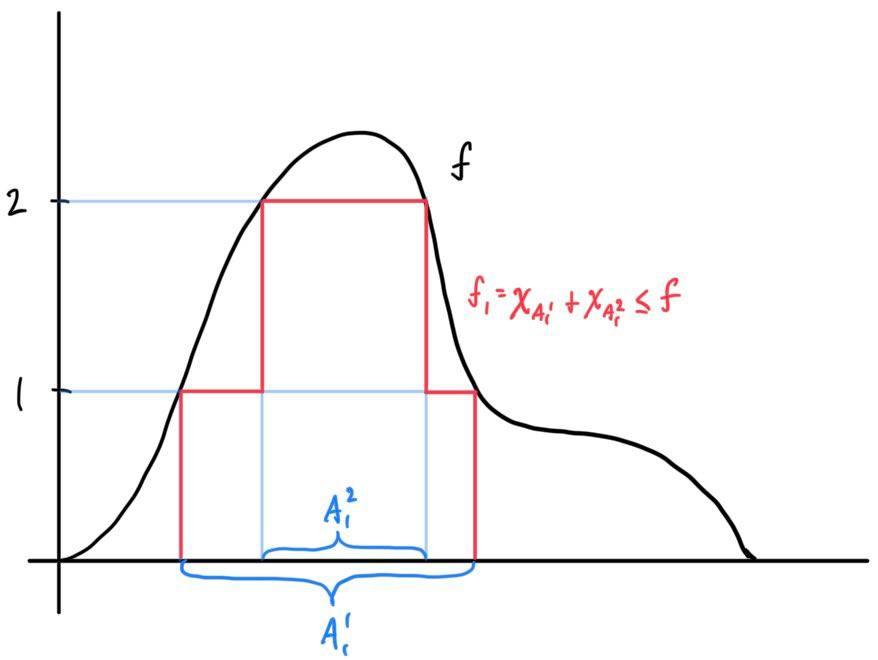
\includegraphics[scale=0.23]{img/Lebesgue_1.jpg}
    \end{center}
    Doing this again with finer subintervals of the codomain gives us, with $f_2 = \chi_{A_2^1} + \chi_{A_2^2} + \chi_{A_2^3} + \chi_{A_2^4} \leq f$. 
    \begin{center}
      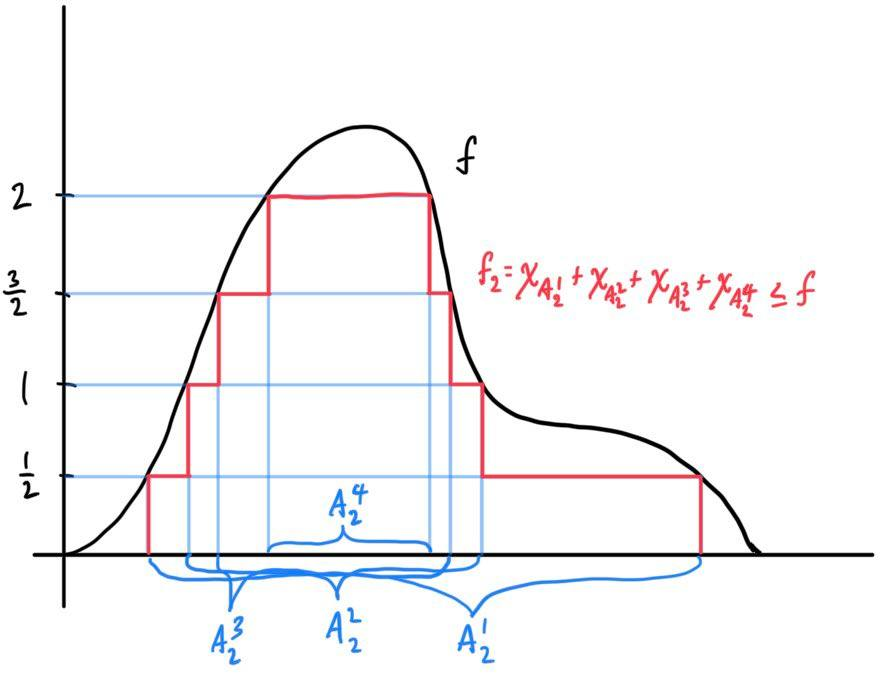
\includegraphics[scale=0.23]{img/Lebesgue_2.jpg}
    \end{center}
    and in general, we have $f_k = \sum_{j=1}^\infty \frac{1}{2^{k-1}} \chi_{A^j_k}$. But we said a simple function is a \textit{finite} sum, and if $\infty$ is in the range of $f$, then this becomes a problem. We can quickly fix this by just truncating the summation at a certain point in the codomain ($f_1$ only considers intervals up to $1$, $f_2$ up to $2$ and so on), ultimately giving us 
    \begin{equation}
      f_k = \sum_{j=1}^{k 2^{k-1}} \frac{1}{2^{k-1}} \chi_{A^j_k} 
    \end{equation}
  \end{proof}


\section{Integration}

  \subsection{Construction of the Riemann Integral}

    We shall first define the integral using the familiar notation of Riemann sums. 

    \begin{definition}[Partitions with Distinguished Points]
      A \textbf{partition} $P$ of a closed interval $[a, b]$, $a < b$, is a finite system of points $x_0, \ldots, x_n$ of the interval such that
      \[a = x_0 < x_1 < x_2 < \ldots < x_n = b\]
      The intervals $[x_{i-1}, x_i]$, $i = 1, 2, \ldots, n$, are called the \textbf{intervals} of the partition $P$. The largest of the lengths of the intervals of the partition $P$, denoted $\lambda(P)$, is called the \textbf{mesh} of the partition. 

      A \textbf{partition with distinguished points} $(P, \xi)$ on the closed interval $[a, b]$ is a partition $P$ of $[a,b]$ along with the set of $n$ points 
      \[\xi_1 \in [x_0, x_1], \xi_2 \in [x_1, x_2], \ldots, \xi_n \in [x_{n-1}, x_n]\]
      The $n$-tuple of $\xi_i$'s is denoted by the single letter $\xi$
      \[\xi = (\xi_1, \xi_2, \ldots, \xi_n)\]
    \end{definition}

    This naturally leads to the following construction. 

    \begin{definition}[Riemann Sums]
      If a function $f$ is defined on a closed interval $[a, b]$ and $(P, \xi)$ is a partition with distinguished points on this closed interval, the sum
      \[\sigma(f; P, \xi) \equiv \sum_{i=1}^n f(\xi_i)\, \Delta x_i, \text{ where } \Delta x_i = x_i - x_{i-1},\]
      is the \textbf{Riemann sum} of the function $f$ corresponding to the partition $(P, \xi)$ with distinguished points on $[a, b]$. 
      \begin{center}
          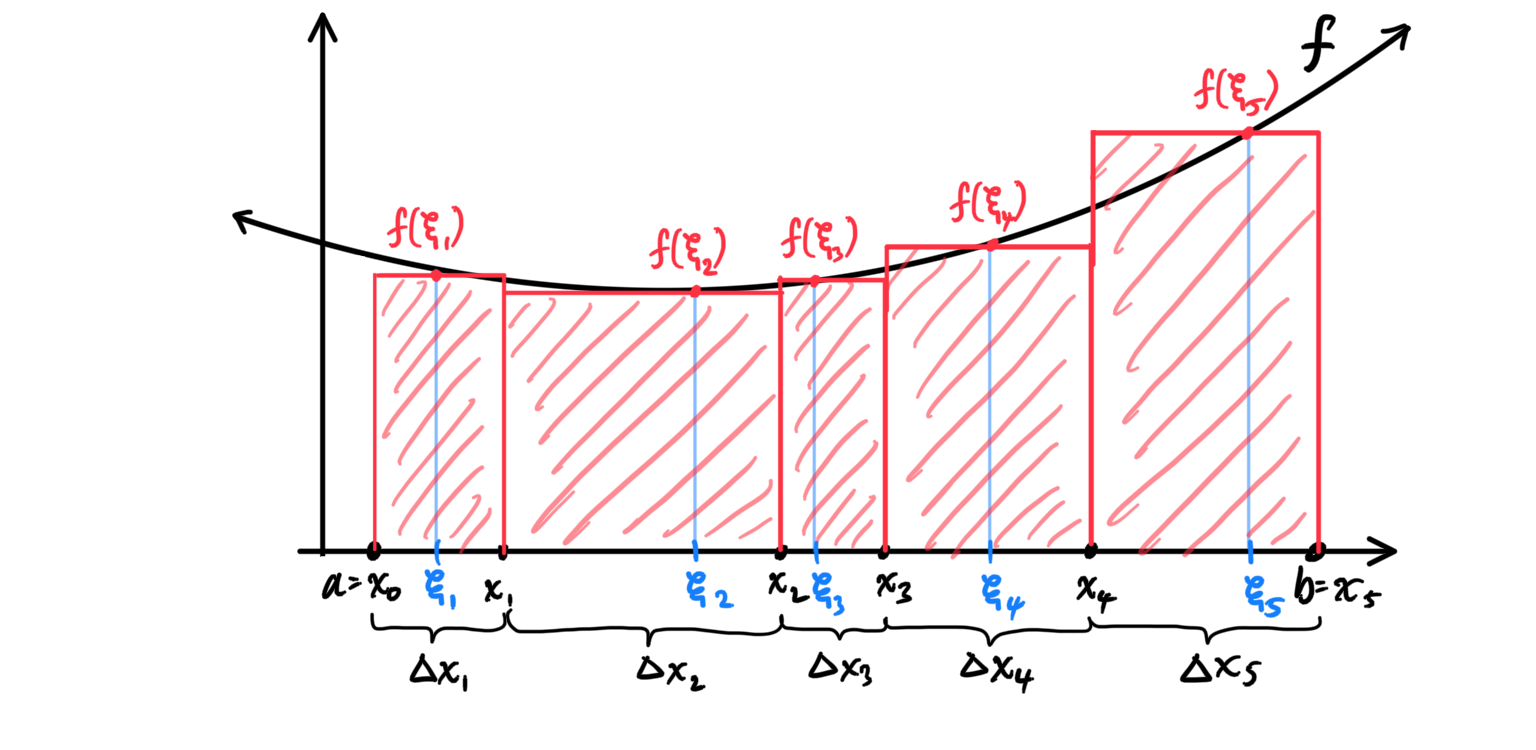
\includegraphics[scale=0.25]{img/Riemann_Sum_with_Partitions_Points.PNG}
      \end{center}
      Thus, when a function $f$ is fixed, the Riemann sum $\sigma (f; P, \xi)$ is a mapping that takes in a partition with distinguished points $p = (P, \xi)$ on the closed interval $[a, b]$ and outputs a number representing the total area of the Riemann sums. That is, for a fixed $f$ and some input $p = (P, \xi)$, we can define the function 
      \[\Phi: \mathcal{P} \longrightarrow \mathbb{R}, \;\;\; \Phi(p) \equiv \sigma(f; p) \equiv \sigma(f; (P, \xi))\]
      that takes in a partition with distinguished points on $[a,b]$ and outputs the corresponding Riemann sum for that fixed $f$. 
    \end{definition}

    \begin{definition}[Riemann Integral]
      The number $\int_a^b f(x)\,dx$ is the \textbf{Riemann integral} of the function $f$ on the closed interval $[a, b]$ if for every $\epsilon>0$ there exists a $\delta>0$ such that
      \[\Bigg| \int_a^b f(x)\,dx - \sum_{i=1}^n f(\xi_i) \Delta x_i \Bigg| < \epsilon\]
      for any partition $(P, \xi)$ with distinguished points on $[a, b]$ whose mesh $\lambda(P)$ is less than $\delta$. We can view this as a limit where $n \rightarrow \infty$, but there is a problem since we can increase the partition within different subsets of $[a,b]$, leading to multiple values of convergence. 
      \begin{center}
          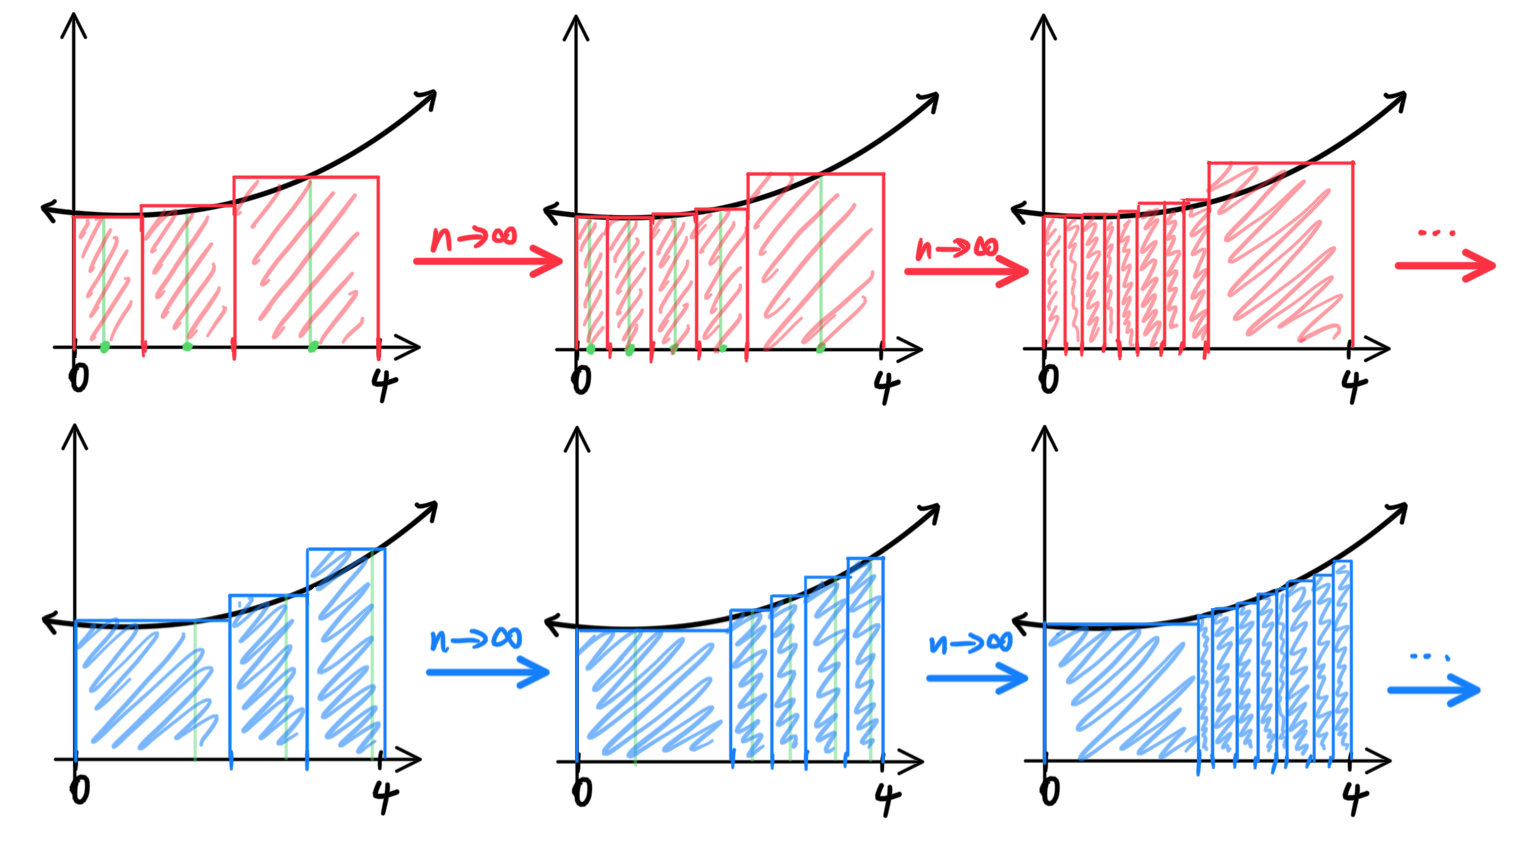
\includegraphics[scale=0.28]{img/Riemann_Integral_Converging_onto_2_Numbers.PNG}
      \end{center}
      Rather, we can set the mesh $\lambda(P)$ to approach $0$, which would take care of the problems. We can visualize this by imagining the lengths of the rectangles converging "uniformly."
      \begin{center}
          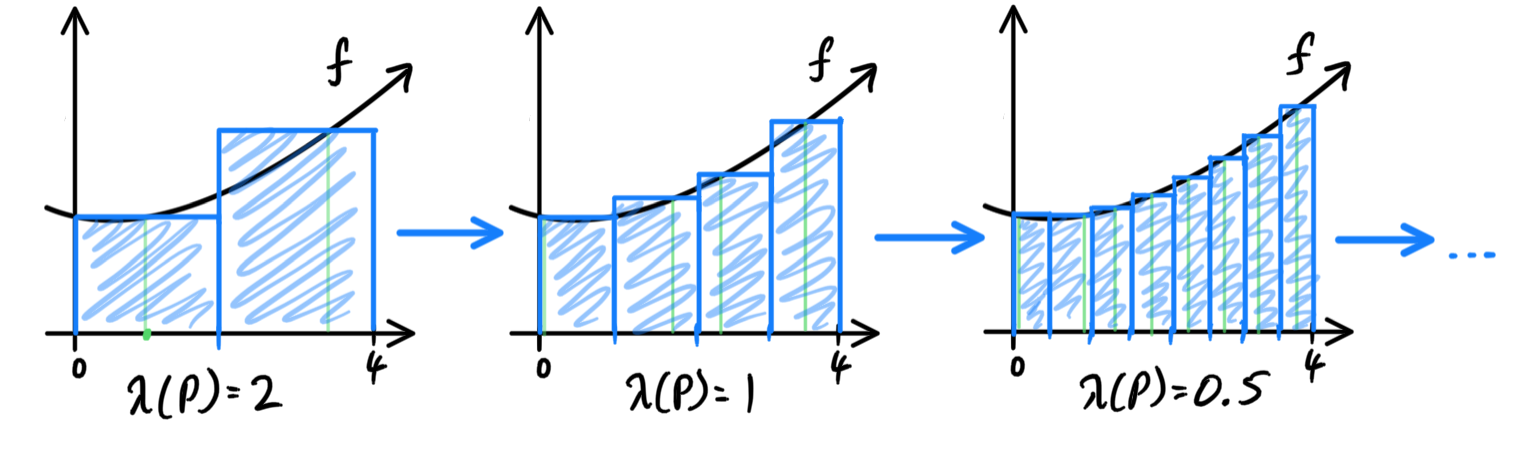
\includegraphics[scale=0.28]{img/Riemann_Integral_Limit_Mesh_goes_to_0.PNG}
      \end{center}
      Therefore, we can culminate by defining the Riemann integral of $f(x)$ over $[a,b]$ as 
      \[\int_a^b f(x)\,dx \equiv \lim_{\lambda(P) \rightarrow 0} \sum_{i=1}^n f(\xi_i) \lambda x_i\]
    \end{definition}

  \subsubsection{Conditions for Integrability}

    \begin{definition}[Riemann Integrable Functions]
      A function $f$ is \textbf{Riemann integrable} on the closed interval $[a, b]$ if 
      \[\int_a^b f(x)\,dx \equiv \lim_{\lambda(P) \rightarrow 0} \sum_{i=1}^n f(\xi_i) \lambda x_i\]
      is defined, i.e. if the limit of the right-hand side of Riemann sums exists as $\lambda(P) \rightarrow 0$ (that is, the Riemann integral of $f$ is defined). 

      Furthermore, the set of Riemann-integrable functions on a closed interval $[a, b]$ is denoted $\mathcal{R}[a,b]$. 
    \end{definition}

    Remember that the Riemann integral, as complicated as the formula is, is still a limit of a function. That means that we can apply the Cauchy criterion to it to determine convergence. 

    \begin{lemma}[Cauchy Criterion on Existence of Riemann Integral]
      Given a function $f$, the integral of $f$ over $[a, b]$, defined
      \[\int_a^b f(x)\,dx \equiv \lim_{\lambda(P) \rightarrow 0} \sum_{i=1}^n f(\xi_i) \lambda x_i\]
      exists if and only if for every $\epsilon>0$, there exists a $\delta>0$ such that 
      \[\big| \sigma(f; P^\prime, \xi^\prime) - \sigma(f; P^{\prime\prime}, \xi^{\prime\prime} \big| < \epsilon\]
      or, what is the same, 
      \[\Bigg| \sum_{i=1}^{n^\prime} f(\xi_i^\prime) \Delta x_i^\prime - \sum_{i=1}^{n^{\prime\prime}} f^(\xi_i^{\prime\prime}) \Delta x_i^{\prime\prime} \Bigg| < \epsilon\]
      for any partitions $(P^\prime, \xi^\prime)$ and $(P^{\prime\prime}, \xi^{\prime\prime})$ with distinguished points on the interval $[a, b]$ with
      \[\lambda(P^\prime), \lambda(P^{\prime\prime}) < \delta\]
      In words, this means that for any $\epsilon>0$ that we choose, there always exists a $\delta>0$ such that \textbf{any} two Riemann sums with mesh size \textbf{both} smaller than $\delta$ will have an error difference of less than $\epsilon$. \begin{center}
          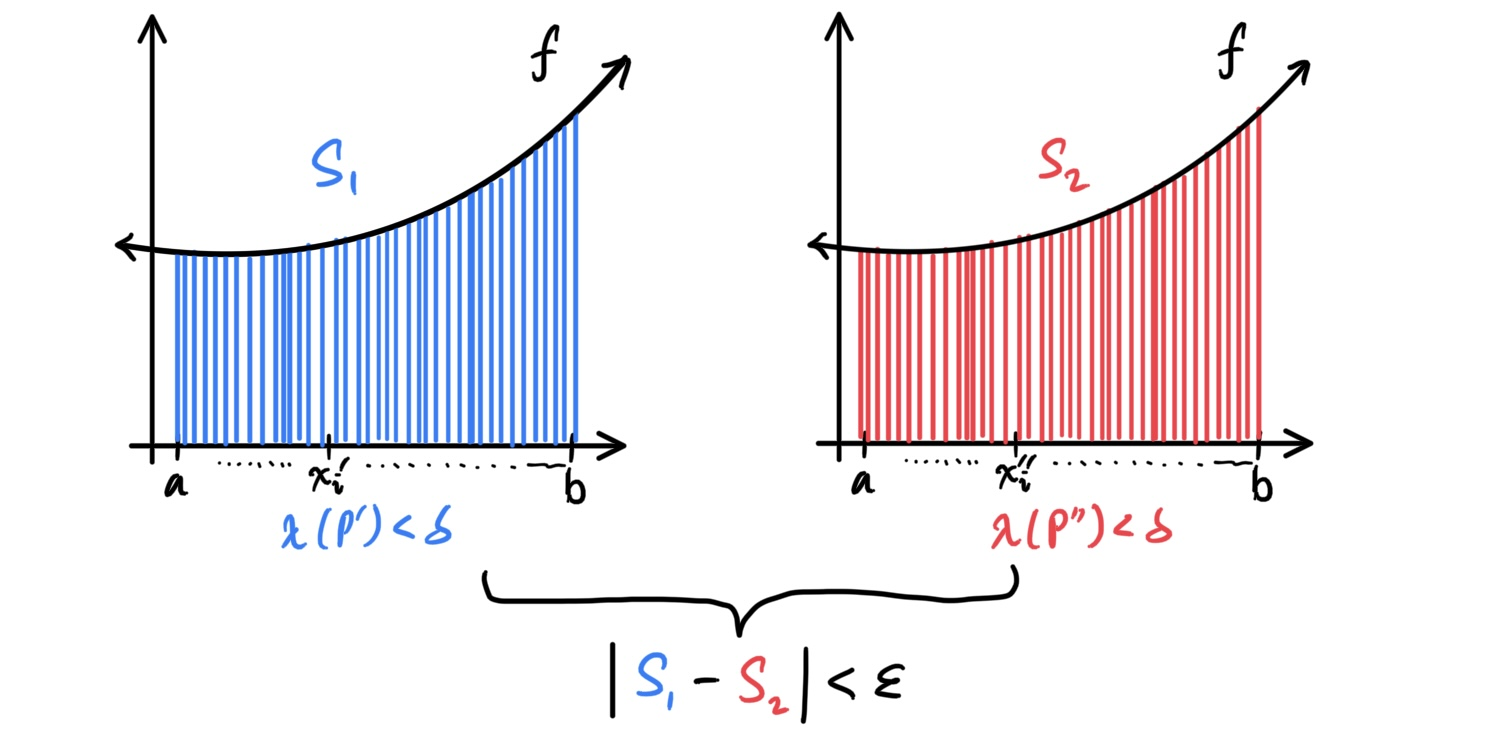
\includegraphics[scale=0.25]{img/Cauchy_Criterion_of_Riemann_Integral.jpg}
      \end{center}
    \end{lemma}

    \begin{theorem}[Necessary Condition for Integrability]
    A necessary condition for $f$ defined on a closed interval $[a, b]$ to be Riemann integrable on $[a, b]$ is that $f$ be bounded on $[a, b]$. That is, 
    \[f \in \mathcal{R}[a, b] \implies f \text{ is bounded on } [a, b]\]
    We can clearly see the necessity of $f$ being bounded by looking at the contrapositive of the following statement. 
    \end{theorem}

    \begin{theorem}[Refinement]
    Given a partition $P$ on interval $[a, b]$, recall that we have points $x_0, \ldots, x_n$ such that
    \[a = x_0 < x_1 < \ldots < x_n = b\]
    Here we introduce new notation: 
    \begin{enumerate}
      \item $\Delta_i$ denotes the interval $[x_{i-1}, x_i]$
      \item $\Delta x_i$ denotes the difference $x_i - x_{i-1}$, i.e. the length of $\Delta_i$
    \end{enumerate}
    If a partition $\Tilde{P}$ of the closed interval $[a, b]$ is obtained from the partition $P$ by the addition of new points to $P$, we call $\Tilde{P}$ a \textbf{refinement} of $P$. 

    When a refinement $\Tilde{P}$ of a partition $P$ is constructed, some (perhaps all) of the closed intervals $\Delta_i = [x_{i-1}, x_i]$ of the partition $P$ themselves undergo partitioning. 
    \[x_{i-1} = x_{i0} < x_{i1} < \ldots < x_{in_i} = x_i\]
    In that connection, it will be useful to label to points of $\Tilde{P}$ by double indices, where in the notation $x_{ij}$ the first index $i$ means that 
    \[x_{ij} \in \Delta_i = [x_{i-1}, x_i]\]
    and the second index $j$ is the ordinal number of the point on the closed interval $\Delta_i = [x_{i-1}, x_i]$. Therefore, it is natural to set the notations
    \begin{enumerate}
      \item $\Delta_{ij} = [x_{i j-1}, x_{ij}]$
      \item $\Delta x_{ij} = x_{ij} - x_{ij-1}$
    \end{enumerate}
    This means that 
    \[\Delta x_i = \Delta x_{i1} + \Delta x_{i2} + \ldots + \Delta x_{in_i}\]
    which can be visualized below
    \begin{center}
      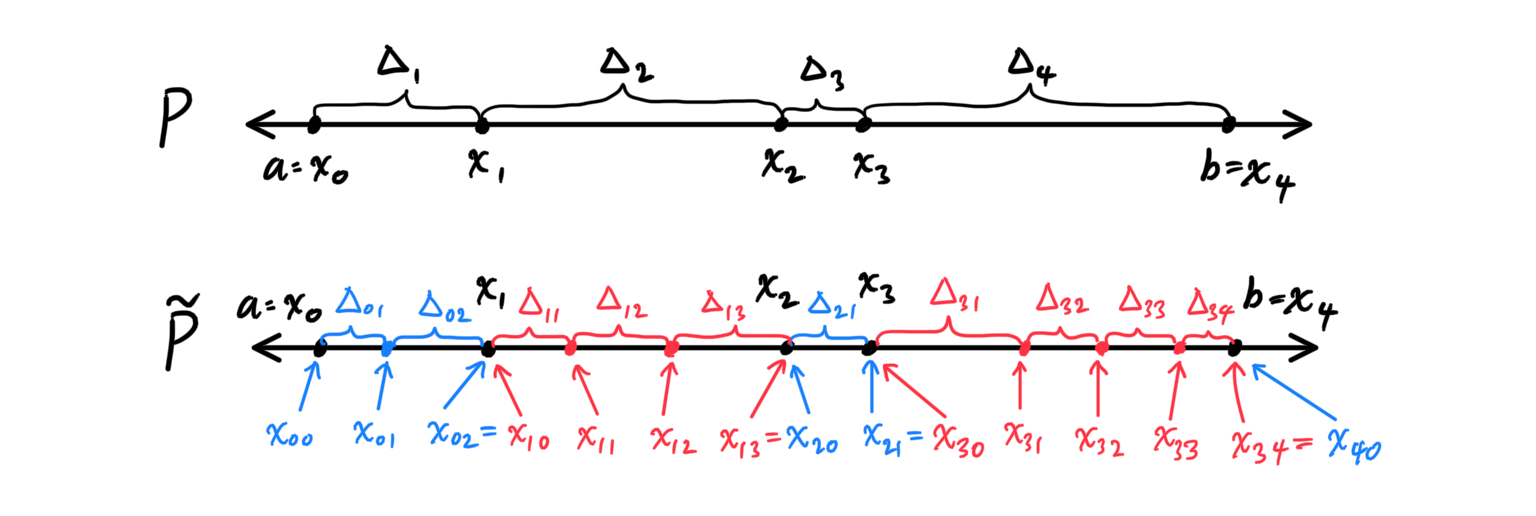
\includegraphics[scale=0.25]{img/Refinement_Definition_Analysis.PNG}
    \end{center}
    \end{theorem}

    \begin{example}[Union of Partitions as a Refinement]
    For some interval $[a, b]$, given partitions $P^\prime$ ($a = x_0 < \ldots < x_n = b$) and $P^{\prime\prime}$ ($a = y_0 < \ldots < y_n = b$), the union of the two partitions $\Tilde{P} = P^\prime \cup P^{\prime\prime}$ is a refinement of both $P^\prime$ and $P^{\prime\prime}$. 
    \begin{center}
        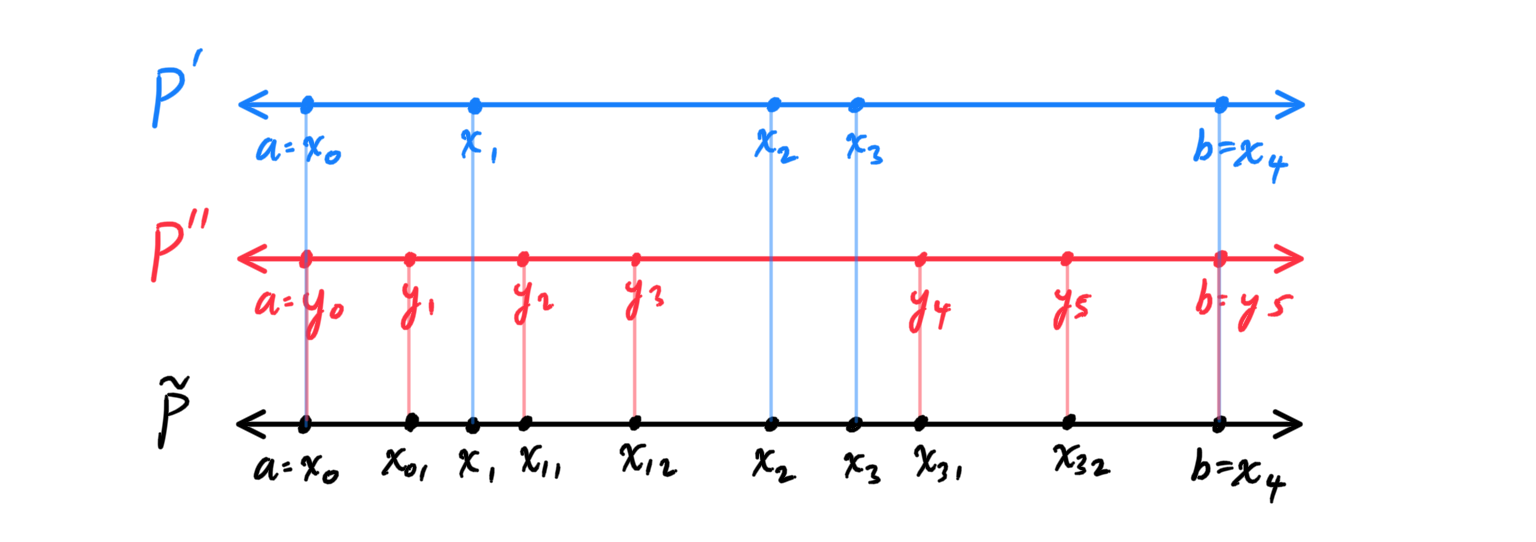
\includegraphics[scale=0.25]{img/Refinement_as_Union_of_Partitions.PNG}
    \end{center}
    \end{example}
    
    Recall that $\omega(f; E)$ denotes the oscillation of the function $f$ on the set $E$; that is, 
    \[\omega(f; E) \equiv \sup_{x^\prime, x^{\prime\prime} \in E} \big| f(x^\prime) - f(x^{\prime\prime})\big|\]
    In particular, $\omega(f; \Delta_i)$ is the oscillation of $f$ on the closed interval $\Delta_i$. 

    \begin{theorem}[Sufficient Condition for Integrability]
    Let $f$ be a bounded on a closed interval $[a, b]$ such that for every $\epsilon > 0$ there exists a number $\delta>0$ such that
    \[\sum_{i=1}^n \omega(f; \Delta_i) \Delta x_i < \epsilon\]
    for any partition $P$ of $[a, b]$ with mesh $\lambda(P) < \delta$. This is equivalent to saying that
    \[\lim_{\lambda(P) \rightarrow 0} \sum_{i = 1}^n \omega (f; \Delta_i) \, \Delta x_i = 0\]
    Then, $f$ is integrable. We can visualize
    \[\sum_{i=1}^n \omega(f; \Delta_i) \Delta x_i\]
    as the following sum of rectangles below. 
    \begin{center}
        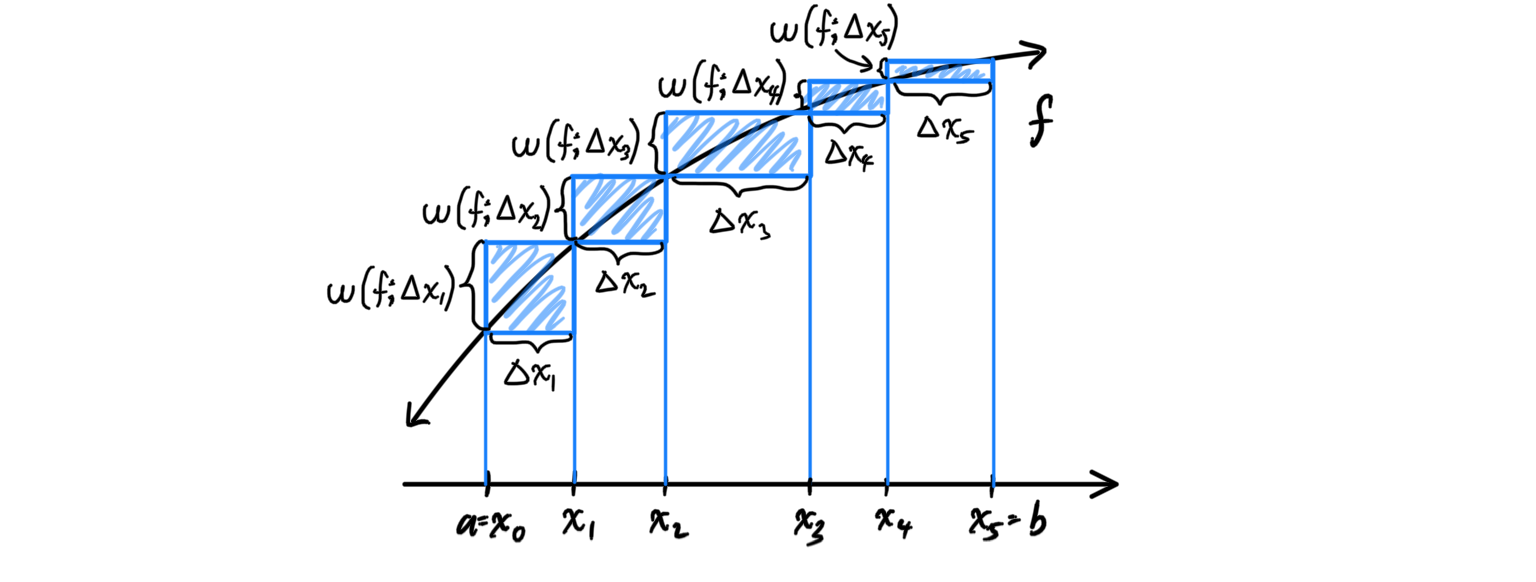
\includegraphics[scale=0.25]{img/Sufficient_Condition_for_Integrability.PNG}
    \end{center}
    What the theorem states, visually, is that as we make all the rectangles smaller and smaller (by putting a limit on the mesh $\lambda(P)<\delta$), we can make the sum of all these rectangles also arbitrarily small. 
    \end{theorem}

    \begin{corollary}[Integrability of Continuous Functions]
    Every continuous function on a closed interval is integrable on that closed interval. That is, 
    \[f \in C[a, b] \implies f \in \mathcal{R}[a, b]\]
    \end{corollary}

    We can actually make a stronger claim. 

    \begin{corollary}[Integrability of Discontinuous Functions]
    If a bounded function $f$ on a closed interval $[a, b]$ is continuous everywhere except at a finite set of points, then $f \in \mathcal{R}[a, b]$. 
    \end{corollary}

    \begin{corollary}[Integrability of Monotonic Functions]
    A bounded monotonic function on a closed interval is integrable on that interval. 
    \begin{center}
        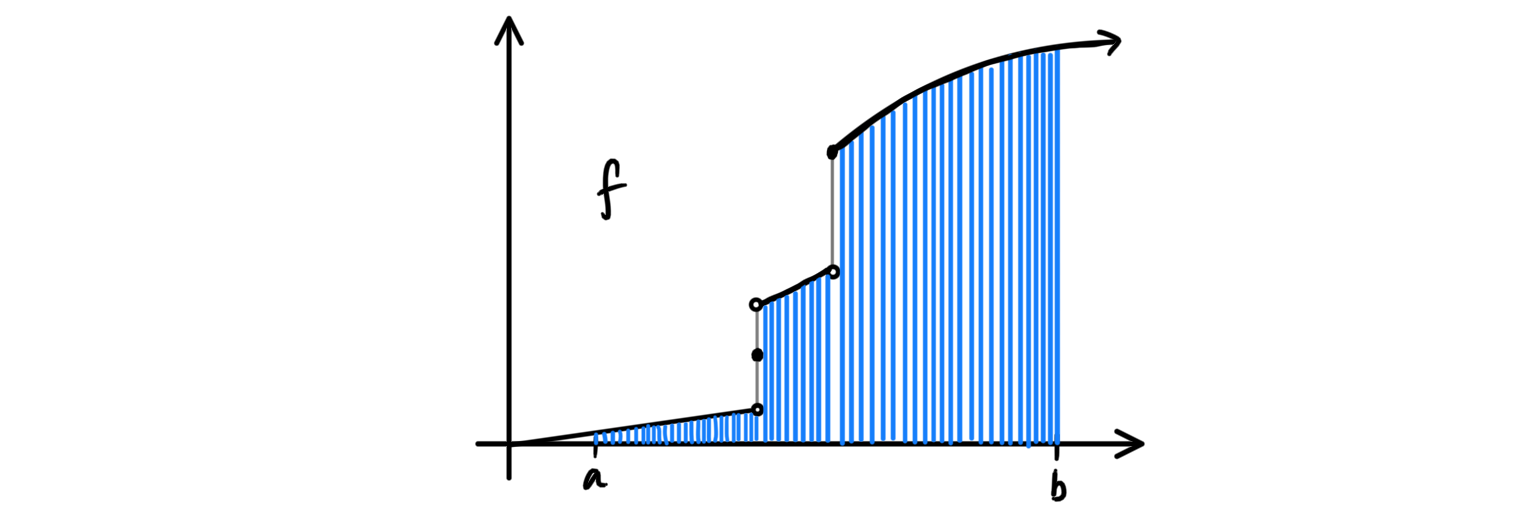
\includegraphics[scale=0.25]{img/Integrability_of_Monotonic_Function.PNG}
    \end{center}
    \end{corollary}

    \begin{definition}[Upper, Lower Riemann Sums]
      Let $f: [a, b] \longrightarrow \mathbb{R}$ be a real-valued function that is defined and bounded on the closed interval $[a, b]$, and let $P$ be a partition of $[a, b]$, and let $\Delta_i$ ($i = 1, 2, \ldots, n$) be the intervals of the partition $P$. Let 
      \begin{align*}
          m_i &= \inf_{x \in \Delta_i} f(x) \\
          M_i &= \sup_{x \in \Delta_i} f(x)
      \end{align*}
      be the infimum and supremum of $f$ over $\Delta x_i$. Then, the sums
      \begin{align*}
          s(f; P) & \equiv \sum_{i = 1}^n m_i \, \Delta x_i \\
          S(f; P) & \equiv \sum_{i=1}^n M_i \, \Delta x_i
      \end{align*}
      are respectively called the \textbf{lower} and \textbf{upper Riemann sums} of the function $f$ on the interval $[a, b]$ corresponding to the partition $P$ of that interval. 

      Given an arbitrary partition $(P, \xi)$ with distinguished points on $[a, b]$, it is clear that
      \[s(f; P) = \inf_{\xi} \sigma(f; P, \xi) \leq \sigma(f; P, \xi) \leq \sup_{\xi} \sigma(f; P, \xi) = S(f; P)\]
    \end{definition}

    \begin{theorem}
    A bounded real-valued function $f: [a, b] \longrightarrow \mathbb{R}$ is Riemann integrable on $[a, b]$ if and only if the following limits exist and are equal to each other. 
    \[\underline{I} \equiv \lim_{\lambda(P) \rightarrow 0} s(f; P) = \lim_{\lambda(P) \rightarrow 0} S(f; P) \equiv \overline{I}\]
    When the relation is true, then the integral is this common value. 
    \[\int_a^b f(x) \,dx = \underline{I} = \overline{I}\]
    \end{theorem}

    Note that this condition of the upper and lower Riemann sums converging to the same value and the condition that 
    \[\lim_{\lambda(P) \rightarrow 0} \sum_{i = 1}^n \omega (f; \Delta_i) \, \Delta x_i = 0\]
    are the same. For we can see that the rectangles visualized from the equation above are the exact same rectangles formed by $S(f; P) - s(f; P)$! 
    \begin{center}
        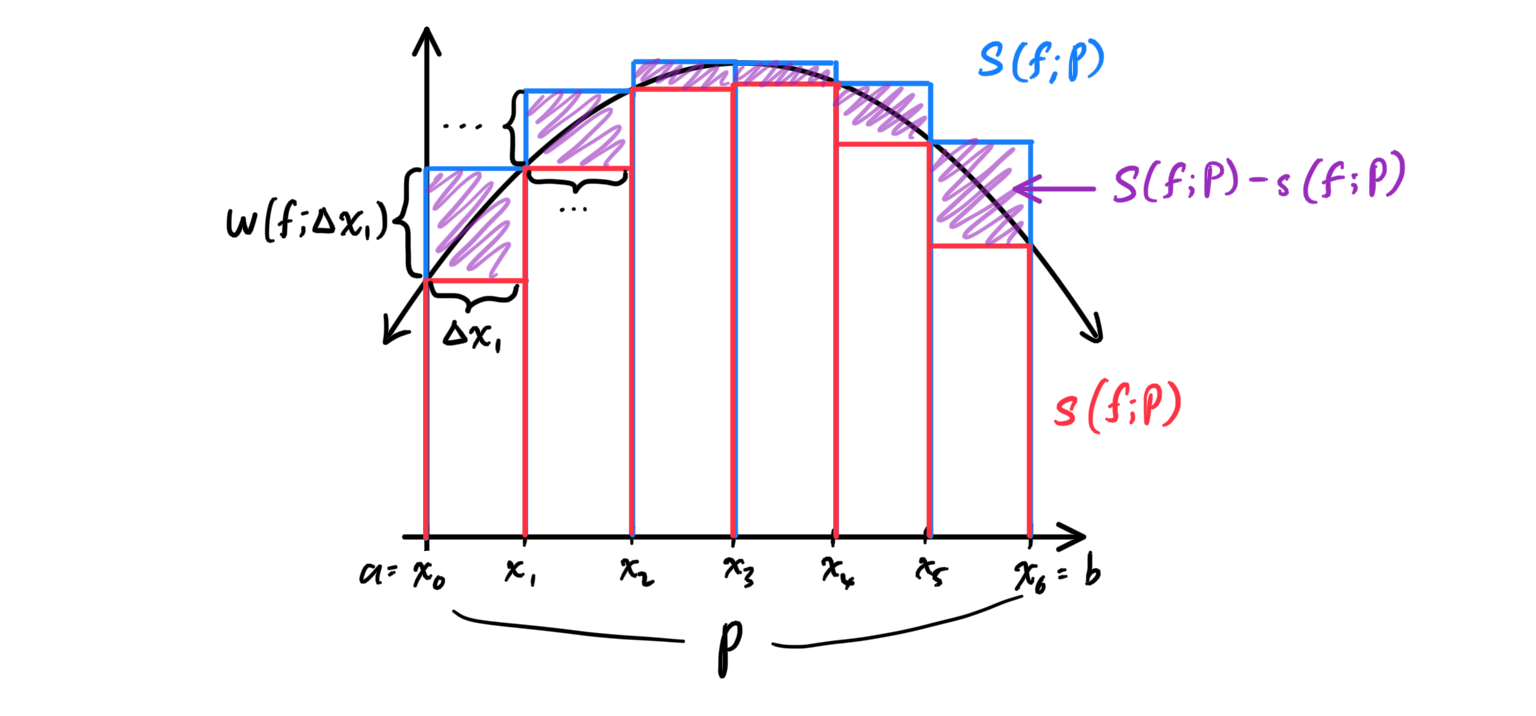
\includegraphics[scale=0.3]{img/Equivalent_Conditions_for_Integrability.PNG}
    \end{center}

    \subsubsection{The Vector Space of Riemann Integrable Functions}

    \begin{theorem}[The Vector Space of Integrable Functions]
    The set of Riemann integrable functions $\mathcal{R}[a, b]$ over closed interval $[a, b]$ is a vector space. That is, given $f, g \in \mathcal{R}[a, b]$ and $\alpha \in \mathbb{R}$, then
    \begin{enumerate}
      \item $(f + g) \in \mathcal{R}[a, b]$ 
      \item $(\alpha f) \in \mathcal{R}[a, b]$
    \end{enumerate}
    Furthermore, 
    \begin{enumerate}
      \item $|f| \in \mathcal{R}[a, b]$
      \item The restriction of $f$ in any $[c, d] \subset [a, b]$, denoted $f \big|_{[c,d]}$, is in $\mathcal{R}[c,d]$
      \item $(f \cdot g) \in \mathcal{R}[a, b]$
    \end{enumerate}
    \end{theorem}
    \begin{proof}

    \end{proof}

    \subsubsection{Lebesgue's Criterion for Riemann Integrability}
    We give Lebesgue's version of an intrinsic description of a Riemann integrable function. 

    \begin{definition}[Measure]
      A set $E \subset \mathbb{R}$ has \textbf{(Lebesgue) measure zero} if for every number $\epsilon > 0$ there exists a covering of the set $E$ be an at most countable system $\{I_k\}$ of intervals, the sum of whose lengths 
      \[\sum_{k=1}^\infty |I_k| \leq \epsilon\]
      This means that the above series summing up the lengths of the intervals is an absolutely convergent series. 
    \end{definition}

    \begin{lemma}
      We can deduce measures of basic sets. 
      \begin{enumerate}
        \item A finite number of points are sets of measure zero. 
        \item The union of a finite or countable number of sets of measure zero is a set of measure zero. \item A subset of a set of measure zero is itself a set of measure zero. 
        \item A closed interval $[a, b]$ with $a<b$ is not a set of measure zero. 
      \end{enumerate}
    \end{lemma}

    \begin{definition}
      If a property holds at all points of a set $X$ except possible the points of a set of measure zero, we say that this property holds \textbf{almost everywhere on $X$} or \textbf{at almost every point of $X$}. 
    \end{definition}

    Now, we can state Lebesgue's criterion for integrability, which nicely summarizes what we have so far. 

    \begin{theorem}[Lebesgue's Criterion for Integrability]
    A function defined on a closed interval is Riemann integrable on that interval if and only if it is bounded and continuous at almost every point. 
    \end{theorem}

    \begin{example}[Non-Integrability of the Dirichlet Function]
    The Dirichlet function
    \[\mathcal{D}(x) \equiv \begin{cases}
    1, & \text{ for } x \in \mathbb{Q} \\
    0, & \text{ for } x \in \mathbb{R} \setminus \mathbb{Q}
    \end{cases}\]
    on the interval $[0,1]$ is not integrable on that interval. We state two different reasons why. 
    \begin{enumerate}
      \item For any partition $P$ of $[0,1]$ we can find in each interval $\Delta_i$ both a rational point $\xi^\prime_i$ and an irrational point $\xi_i^{\prime\prime}$. Then, we can see that the lower and upper Riemann sums do not necessarily converge to each other since
      \[\sigma(f; P, \xi^\prime) = \sum_{i=1}^n 1 \cdot \Delta x_i = 1 \text{ while } \sigma(f;P, \xi^{\prime\prime}) = \sum_{i=1}^n 0 \cdot \Delta x_i = 0\]
      as $\lambda(P) \rightarrow 0$. 
      \item From the point of view of the Lebesgue criterion the nonintegrability of the Dirichlet function is obvious since $\mathcal{D}(x)$ is discontinuous at every point of $[0, 1]$, which is not a set of measure zero. 
    \end{enumerate}
    \end{example}

    Notice that by the Lebesgue criterion, integrability is a weaker condition than continuity. That is, 
    \[f \text{ continuous } \implies f \text{ Riemann integrable}\]
    but not necessarily the other way around. It turns out that this has consequences when determining the composition of functions. 

    \begin{proposition}[Integrable + Continuous Composition]
    Let $f: I_1 = [a, b] \longrightarrow\mathbb{R}$ be a function that is integrable on $[a, b]$, with Im$\,f = [c, d] = I_2$. Define a continuous (remember, continuity is stronger than integrability) function $g: [c, d] \longrightarrow \mathbb{R}$. Then the composition
    \[g \circ f: [a, b] \longrightarrow \mathbb{R}\]
    is clearly defined and continuous at all the points of $[a, b]$ where $f$ is continuous. But since $f$ is integrable, the union of all the discontinuities in $[a, b]$ must have measure zero, and so it follows that since $[a, b]$ is the same  
    \[g \circ f \in \mathcal{R}[a, b]\]
    Therefore, we can found out that 
    \[f \text{ integrable and } g \text{ continuous} \implies g \circ f \text{ integrable}\]
    as visualized in the commutative diagram below. 
    \[
      \begin{tikzcd}
        I_1 \arrow[r, "f"] \arrow[rr, bend left, "g \circ f"] & I_2 \arrow[r, "g"] & \mathbb{R}
      \end{tikzcd}
    \]
    However, contrary to intuition, 
    \[f \text{ integrable and } g \text{ integrable} \centernot\implies g \circ f \text{ integrable}\]
    \end{proposition}

    We present a counterexample. 
    \begin{example}
    Consider the functions
    \[|sgn|(x) \equiv \begin{cases}
    1 & x \neq 0 \\
    0 & x = 0
    \end{cases}\]
    and the Riemann function 
    \[\mathcal{R}(x) \equiv \begin{cases}
    \frac{1}{n} & x = \frac{m}{n} \in \mathbb{Q}, \gcd(m, n) = 1 \\
    0 & x \in \mathbb{R} \setminus \mathbb{Q}
    \end{cases}\]
    We can see that $\mathcal{R}$ is continuous at all irrational points and discontinuous at all rational points except $0$, meaning that it is integrable ($\mathbb{Q}$ has measure zero). Then, the composition of these two functions is precisely the Dirichlet function
    \[\mathcal{D}(x) = |sgn| \circ \mathcal{R}\]
    which is not integrable. 
    \end{example}

  \subsection{Basic Properties of the Integral}

    One of the most basic properties of the integral is that it is a linear map. 
    \begin{lemma}[Linearity of the Integral]
      Given closed interval $[a, b] \subset \mathbb{R}$, the Riemann integration function 
      \[\int_a^b: \mathcal{R}[a, b] \longrightarrow \mathbb{R}\]
      is a linear functional living within the dual space $\mathbb{R}^* [a, b]$. That is, given $f, g \in \mathcal{R}[a, b]$, a linear combination of them $\alpha f + \beta g$ is also integrable on $[a,b]$, and 
      \[\int_a^b (\alpha f + \beta g)(x)\,dx = \alpha \int_a^b f(x)\,dx + \beta \int_a^b g(x)\,dx\]
    \end{lemma}
    \begin{proof}
    It is clear from basic algebraic transformation that the Riemann sums for the integral expressions on both sides are equal. 
    \[\sum_{i=1}^n (\alpha f + \beta g) (\xi_i) \Delta x_i = \alpha \sum_{i=1}^n f(\xi_i) \Delta x_i + \beta \sum_{i=1}^n g(\xi_i) \Delta x_i\]
    Taking the limit as $\lambda(P) \rightarrow 0$ on both sides leads to the respective Riemann integrals. 
    \end{proof}


    The next property of the Riemann integral is its additive property \textbf{on the interval of integration}. Note that the value of the integral 
    \[\int_a^b f(x) \,dx \equiv \lim_{\lambda(P) \rightarrow 0} \sigma(f; P, \xi)\]
    depends on both the integrand and the closed interval over which the integral is taken. 

    \begin{lemma}[Properties of the Interval of Integration]
      If $a < b < c$ and $f \in \mathcal{R}[a, c]$, then $f \big|_{[a,b]} \in \mathcal{R}[a, b]$, $f \big|_{[b,c]} \in \mathcal{R}[b, c]$, and the following equality holds 
      \[\int_a^c f(x)\,dx = \int_a^b f(x)\, dx + \int_b^c f(x)\,dx\]
      From these we set
      \[\int_a^b f(x)\,dx \equiv - \int_b^a f(x)\,dx\]
      and 
      \[\int_a^a f(x)\,dx \equiv 0\]
    \end{lemma}

    \begin{theorem}[Symmetry of the Riemann Integral]
    Let $a, b, c \in \mathbb{R}$ and let $f$ be integrable over the largest closed interval having two of these points as endpoints. Then, the restriction of $f$ to each of the other closed intervals is also integrable over those intervals and the following equality holds. 
    \[\int_a^b f(x)\,dx + \int_b^c f(x)\,dx + \int_c^a f(x)\,dx = 0\]
    This property can be abstractified to those of additive interval functions, which will be shown soon. 
    \end{theorem}

    We finally end with an important property of the integral which, as seen later, allows us to define inner products on function spaces. 
    \begin{theorem}
    If $a \leq b$ and $f \in \mathcal{R}[a, b]$, then $|f| \in \mathcal{R}[a, b]$, and 
    \[\Bigg| \int_a^b f(x)\,dx \Bigg| \leq \int_a^b |f|(x)\,dx\]
    \end{theorem}

    \subsubsection{Mean Value Theorem of the Integral}

    \begin{lemma}[Monotonicity of the Integral]
      If $a \leq b, f_1, f_2 \in \mathcal{R}[a, b]$, and $f_1 (x) \leq f_2 (x)$ for every $x \in [a, b]$, then
      \[\int_a^b f_1 (x)\,dx \leq \int_a^b f_2 (x)\,dx\]
      \begin{center}
          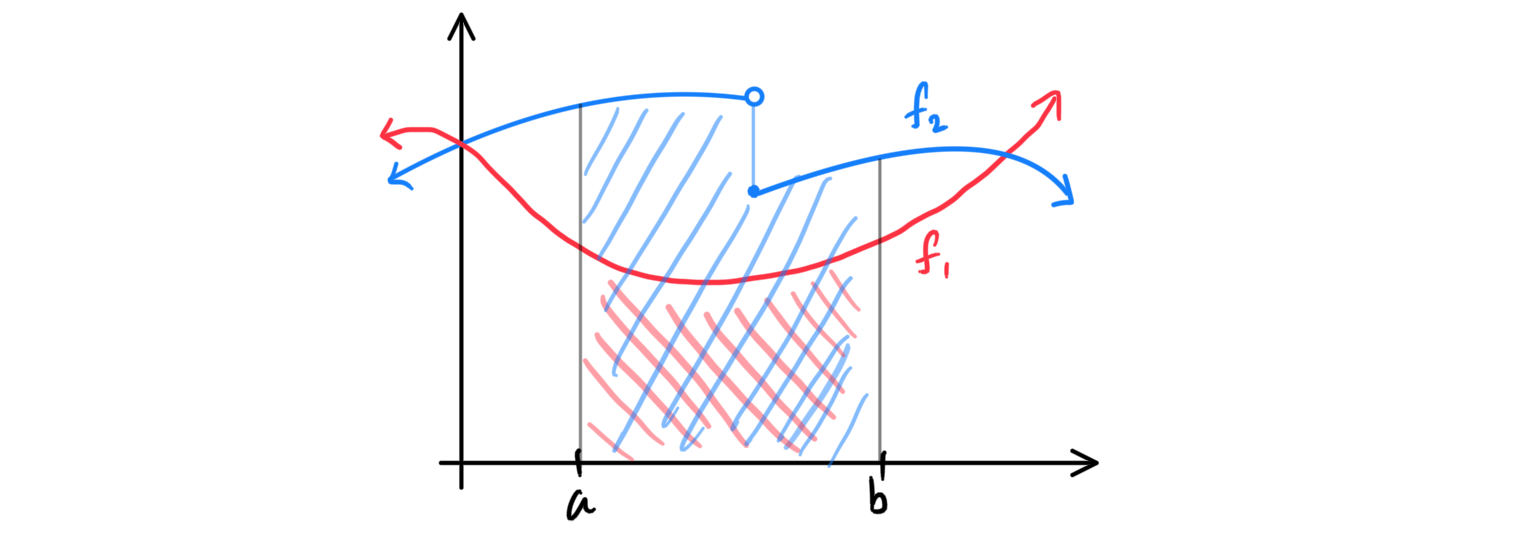
\includegraphics[scale=0.27]{img/Monotonicity_of_Integral.PNG}
      \end{center}
      This immediately implies that given constants $m, M$ such that $m \leq f(x) \leq M$ at each $x \in [a, b]$, we have
      \[m \cdot (b - a) \leq \int_a^b f(x)\,dx \leq M \cdot (b-a)\]
      This is very easily visualized below. 
      \begin{center}
          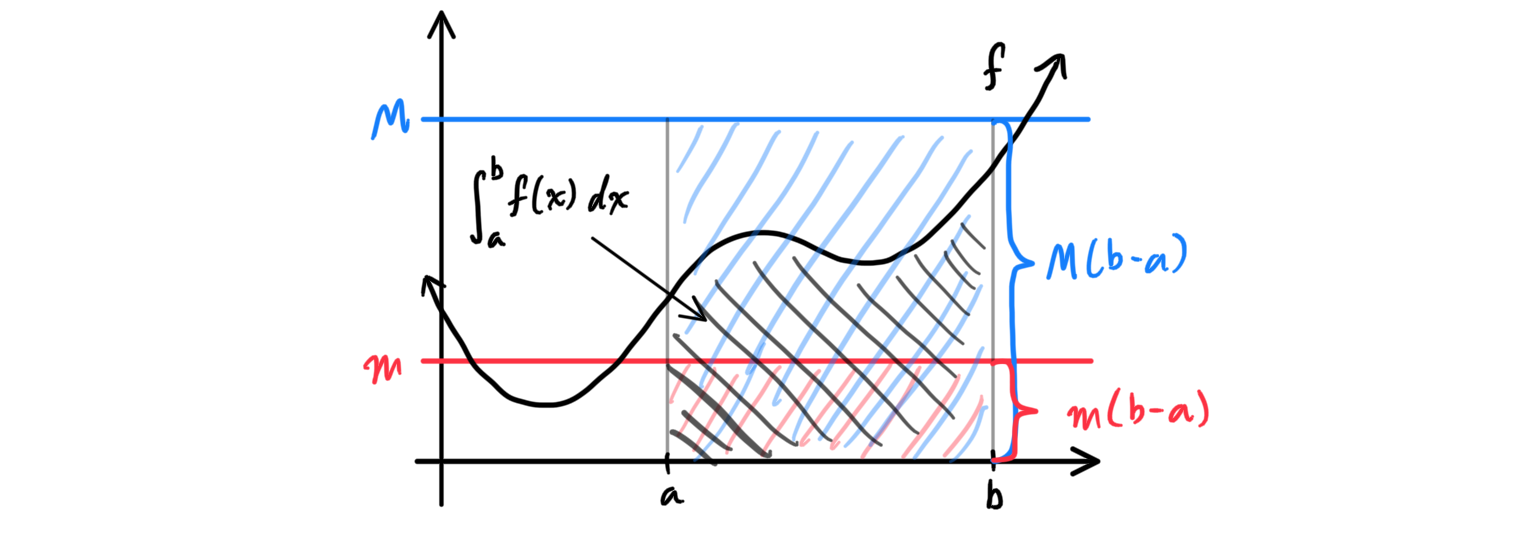
\includegraphics[scale=0.27]{img/Monotonicity_of_Intergral_2.PNG}
      \end{center}
      In particular, if $0 \leq f(x)$ on $[a, b]$, then
      \[0 \leq \int_a^b f(x)\,dx\]
    \end{lemma}

    \begin{theorem}[Mean Value Theorem of the Integral]
    Given $f \in \mathcal{R}[a, b]$, with 
    \[m = \inf_{x \in [a, b]} f(x) \text{ and } M = \sup_{x \in [a, b]} f(x)\]
    then there exists a number $\mu \in [m, M]$ such that
    \[\int_a^b f(x)\,dx = \mu \cdot (b - a)\]
    Furthermore, if $f \in C[a, b]$ (that is, continuous on $[a, b]$), it immediately follows by the intermediate value theorem that there exists a point $\xi \in [a, b]$ such that
    \[\int_a^b f(x)\,dx = f(\xi) (b - a)\]
    \begin{center}
        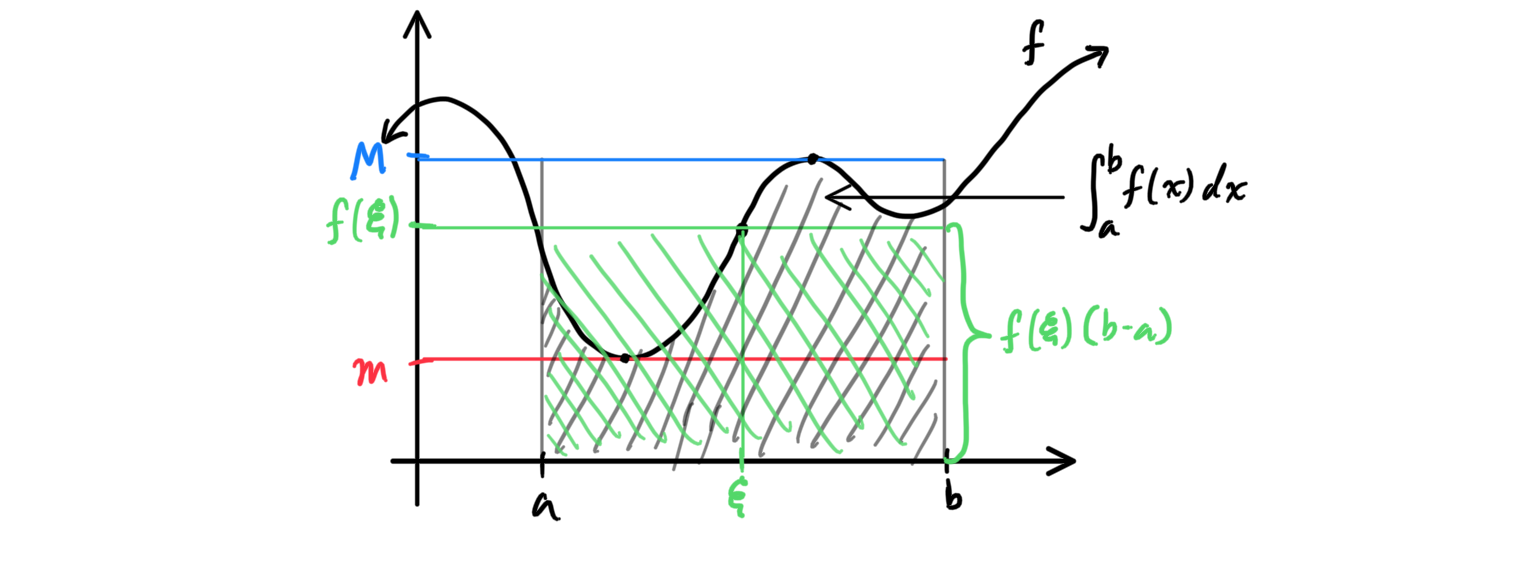
\includegraphics[scale=0.27]{img/Mean_Plus_Intermediate_Value_Theorem_Integral.PNG}
    \end{center}
    \end{theorem}

    Due to the length of the proof, we ask the reader to take it for granted the following theorem. 

    \begin{theorem}[Bonnet's Formula]
    If $f, g \in \mathcal{R}[a, b]$ and $g$ is a monotonic function on $[a, b]$, then there exists a point $\xi \in [a, b]$ such that
    \[\int_a^b (f \cdot g) (x)\,dx = g(a) \int_a^\xi f(x)\,dx + g(b) \int_\xi^b f(x)\,dx\]
    \end{theorem}

  \subsection{Connections between Integrals, Primitives, Derivatives}

    \begin{definition}[Integral with Variable Upper Limit]
      Let $f \in \mathcal{R}[a, b]$, and let us choose an $x \in [a, b]$ in order to construct the function
      \[F(x) \equiv \int_a^x f(t)\,dt\]
      which is called an \textbf{integral with variable upper limit}. Note that since $[a, x] \subset [a, b]$, it follows that $f \big|_{[a,x]} \in \mathcal{R}[a, x]$ and therefore the function $x \mapsto F(x)$ is unambiguously defined for $x \in [a, b]$. 
      \begin{center}
          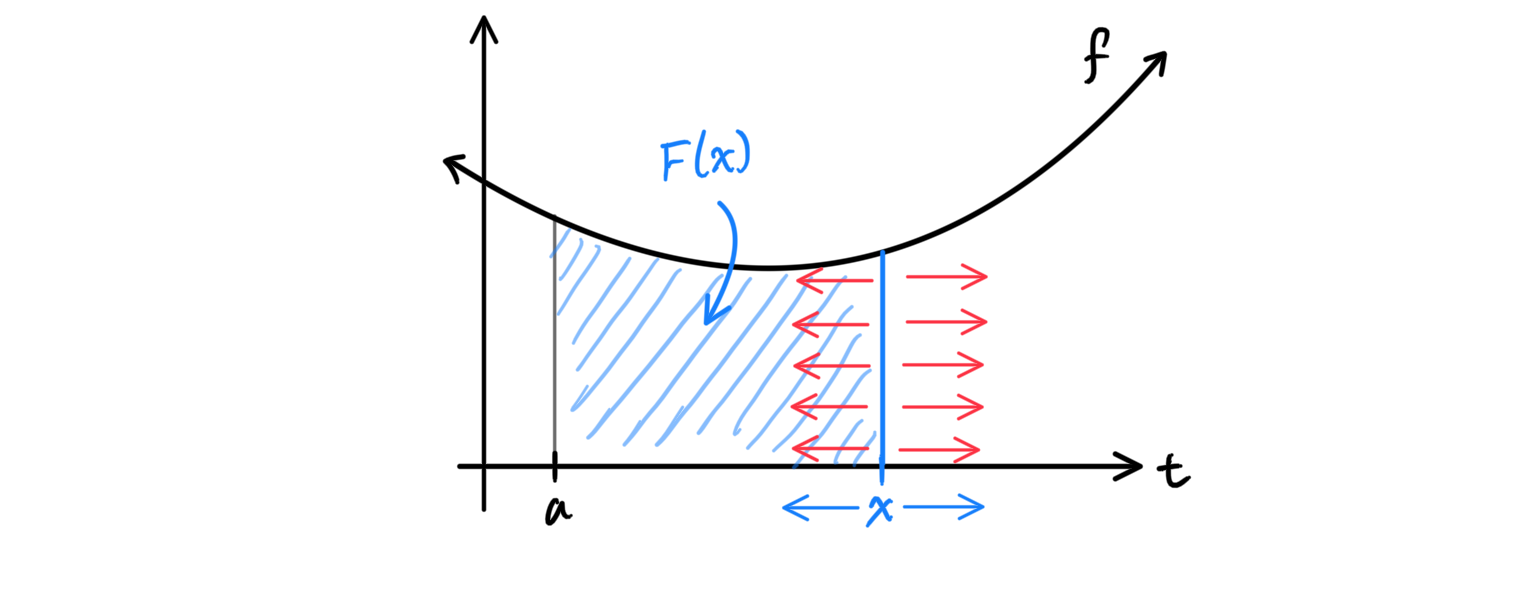
\includegraphics[scale=0.27]{img/Integral_with_Variable_Upper_Limit.PNG}
      \end{center}
      Furthermore, $F(x)$ is continuous on $[a, b]$. Since $f$ is integrable on $[a, b]$, it is bounded by a constant $C$ such that
      \[|f(t)| \leq C \text{ on } [a, b]\]
      It follows from the additive properties of the integral and boundedness theorem that 
      \[|F(x + h) - F(x)| \leq C|h|\]
      if $x, x + h \in [a, b]$, as visualized. This means that for any $\delta$-neighborhood of $F(x)$, we can find an arbitrary small $h$ such that the $C|h|$-neighborhood of $F(x)$ is completely contained in the $\delta$-neighborhood. But by the inequality above, this means that there exists an $\epsilon = h$-neighborhood of $x$ such that its entire image is contained within the $C|h|$-neighborhood, which itself is contained within the $\delta$-neighborhood. This shows that $F$ is continuous. 
    \end{definition}

    \begin{theorem}[First Fundamental Theorem of Calculus]
    Let $f \in \mathcal{R}[a, b]$ be continuous at point $x \in [a, b]$ (resp. continuous on closed interval $[a, b]$). Let $F$ be the function, defined for all $x \in [a, b]$ by 
    \[F(x) \equiv \int_a^x f(t)\,dt\]
    Then, $f$ is continuous and differentiable at $x$ (resp. uniformly continuous on $[a, b]$ and differentiable on $(a, b)$), 
    \[F^\prime (x) = f(x)\]
    at $x$ (resp. for all $x \in [a, b]$). This is an amazing fact, because visually, it tells us that the rate at which the integral $F$ is increasing at $x$ (represented by the increasing area under the curve of $f$) is equal to the value of $f$ at the point $x$ itself! 
    \begin{center}
        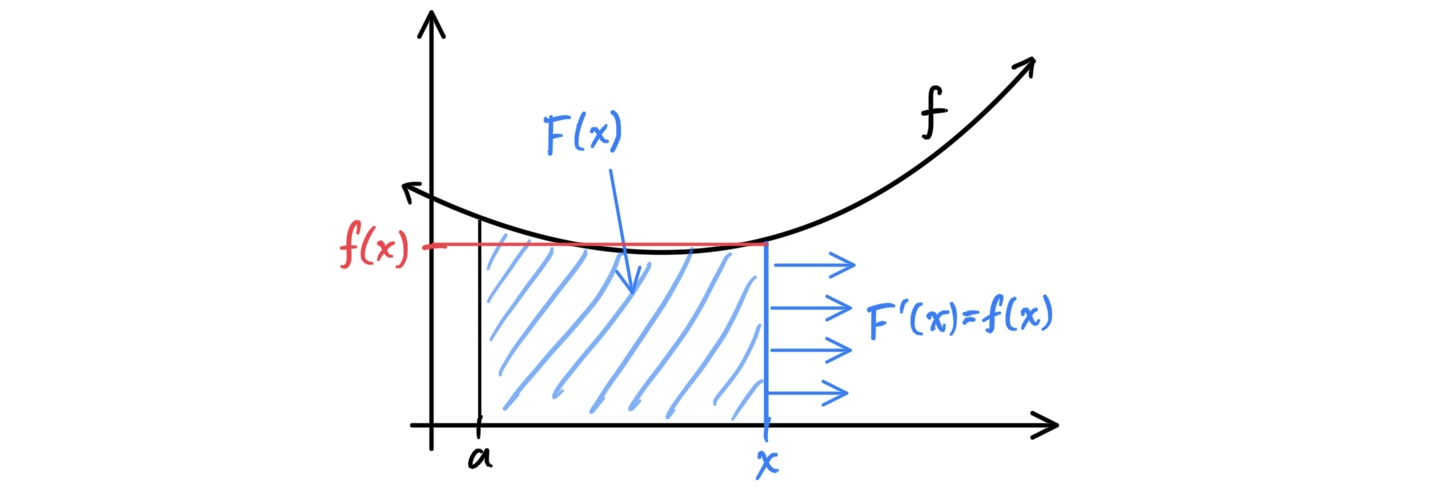
\includegraphics[scale=0.25]{img/First_Fundamental_Theorem_Analysis.jpg}
    \end{center}
    \end{theorem}
    \begin{proof}
    Let $x, x + h \in [a, b]$, and let us estimate the difference $F(x+h) - F(x)$. It follows from the continuity of $f$ at $x$ that $f(t) = f(x) + \Delta(t)$, where $\Delta(t) \rightarrow 0$ as $t \rightarrow x$. If point $x$ is held fixed, the function 
    \[\Delta(t) = f(t) - f(x)\]
    is integrable on $[a, b]$, being the difference of the integrable function $t \mapsto f(t)$ and the constant $f(x)$. Let us denote
    \[M(h) \equiv \sup_{t \in [x, x+h]} |\Delta(t)|\]
    which means that $M(h)$ is the largest difference between $f(x)$ and $f(t)$ in the interval $[x, x+h]$. 
    \begin{center}
        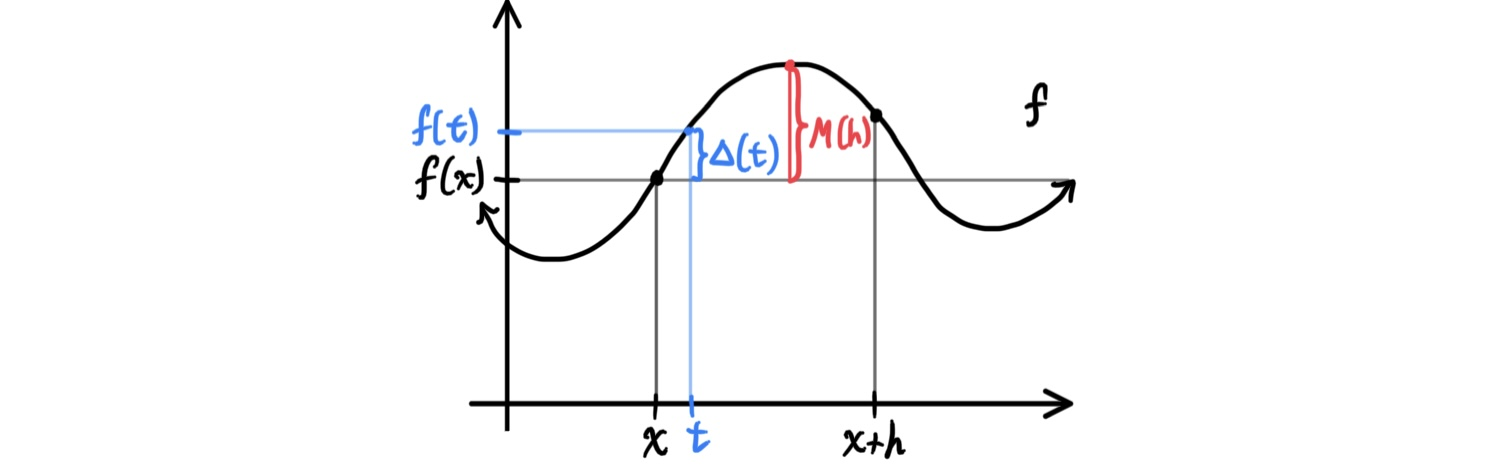
\includegraphics[scale=0.25]{img/Proof_First_Fundamental_Theorem_Analysis.jpg}
    \end{center}
    Clearly $M(h) \rightarrow 0$ as $h \rightarrow 0$. We can now find
    \begin{align*}
        F(x + h) - F(x) & = \int_a^{x+h} f(t)\,dt - \int_a^x f(t)\,dt \\
        & = \int_x^{x+h} f(t)\,dt \\
        & = \int_x^{x+h} \big( f(x) + \Delta(t)\big)\,dt \\
        & = \int_x^{x+h} f(x)\,dt + \int_x^{x+h} \Delta(t)\,dt \\
        & = f(x) h + \alpha(h) h
    \end{align*}
    where we have set 
    \[\int_x^{x+h} \Delta(t)\,dt = \alpha(h) h\]
    where $\alpha$ is infinitesimal as $h \rightarrow 0$, since 
    \[\Bigg| \int_x^{x+h} \Delta(t)\,dt \Bigg| \leq \Bigg| \int_x^{x+h} |\Delta(t)|\,dt \Bigg| \leq \Bigg| \int_x^{x+h} M(h)\,dt \Bigg| = M(h) |h| = \alpha(h)|h|\]
    Therefore, we have shown that if the function $f$ is continuous at a point $x \in [a, b]$, then for displacements $h$ from $x$ such that $x +h \in [a, b]$, the following equality holds.
    \[F(x + h) - F(x) = f(x) h + \alpha(h) h\]
    where $\alpha(h) \rightarrow 0$ as $h \rightarrow 0$, and by definition, this means that $F(x)$ is differentaible on $[a, b]$ at the point $x \in [a, b]$ and that $F^\prime(x) = f(x)$. 
    \end{proof}

    \begin{corollary}
    Every bounded function $f: [a, b] \longrightarrow \mathbb{R}$ on the closed interval $[a, b]$ and has only a finite number of points of discontinuity has a primitive, and every primitive of $f$ on $[a, b]$ has the form 
    \[\mathcal{F}(x) \equiv \int_a^x f(t)\,dt + c\]
    where $c$ is a constant. 
    \end{corollary}

    \begin{theorem}[Second Fundamental Theorem of Calculus]
    Let $f$ be a real-valued function on a closed interval $[a, b]$ with $\mathcal{F}$ any primitive of $f$ on $[a, b]$. If $f$ is Riemann-integrable (i.e. $f$ bounded with finite points of Lebesgue measure zero) on $[a, b]$, then 
    \[\int_a^b f(x)\,dx  = \mathcal{F} \big|_a^b \equiv \mathcal{F}(b) - \mathcal{F}(a)\]
    \begin{center}
        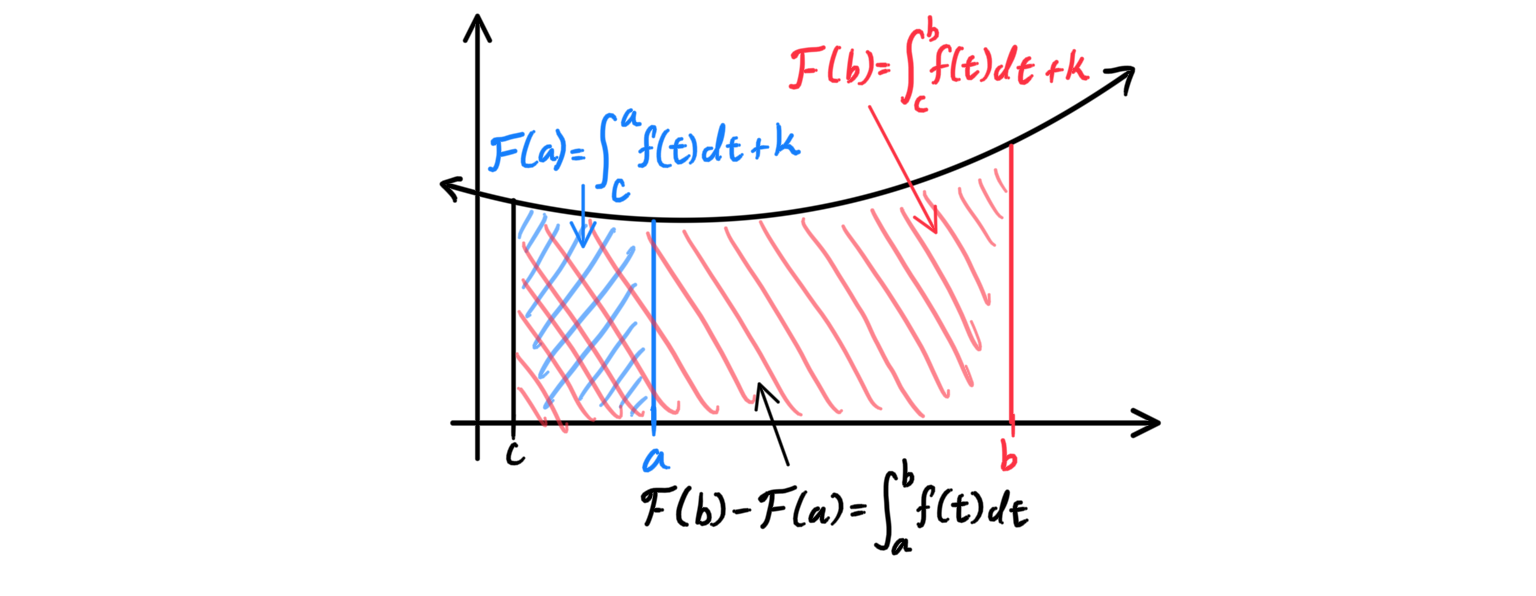
\includegraphics[scale=0.25]{img/Second_Fundamental_Theorem_Analysis.PNG}
    \end{center}
    \end{theorem}
    \begin{proof}
    We already know that a bounded function on a closed interval having a finite number of discontinuities is integrable, and by the corollary, we are guaranteed an existence of a primitive $\mathcal{F}(x)$ of the function $f$ on $[a, b]$ with the form 
    \[\mathcal{F} (x) \equiv \int_a^x f(t)\,dt + c\]
    Setting $x = a$, we find that $c = \mathcal{F}(a)$, and so 
    \[\mathcal{F}(x) \equiv \int_a^x f(t)\,dt + \mathcal{F}(a)\]
    Evaluating $\mathcal{F}$ at $x = b$ gives
    \[\int_a^b f(t)\,dt = \mathcal{F}(b) - \mathcal{F}(a)\]
    \end{proof}

    \subsubsection{Integration by Parts and Taylor's Formula}
    \begin{theorem}[Definite Integration by Parts]
    If the functions $u(x)$ and $v(x)$ are continuously differentiable on a closed interval with endpoints $a$ and $b$, then
    \[\int_a^b (u \cdot v^\prime)(x)\,dx = (u \cdot v)\big|^b_a - \int_a^b (v \cdot u^\prime)(x)\,dx\]
    which is customarily written in the form as
    \[\int_a^b u\,dv = u \cdot v \big|_a^b - \int_a^b v\,du\]
    \end{theorem}
    \begin{proof}
    By the product rule of differentiation, we have
    \[(u \cdot v)^\prime (x) = (u^\prime \cdot v)(x) + (u \cdot v^\prime) (x)\]
    where by hypothesis, $u^\prime \cdot v, u \cdot v^\prime$ are continuous and hence integrable on $[a, b]$. Using the linearity of the integral and the 2nd fundamental theorem of calculus, we get
    \[(u \cdot v) (x) \big|^b_a = \int_a^b (u^\prime \cdot v)(x)\,dx + \int_a^b (u \cdot v^\prime) (x)\,dx\]
    \end{proof}

    \begin{theorem}[Integral Form of the Remainder]
    If $f: E \longrightarrow \mathbb{R}$ has continuous derivatives up to order $n$ on the closed interval $[a, x]$, then Taylor's formula holds
    \[f(x) = f(a) + \frac{f^\prime (a)}{1!} (x - a) + \ldots + \frac{f^{(n-1)}(a)}{(n-1)!} (x - a)^{n-1} + r_{n-1}(a; x)\]
    where 
    \[r_{n-1} (a;x) = \frac{1}{(n-1)!} \int_a^x f^{(n)} (t) (x - t)^{n-1} \,dt\]
    This form is called \textbf{Taylor's formula with the integral form of the remainder}. 
    \end{theorem}
    \begin{proof}
    Using the 2nd fundamental theorem and the definite integration by parts formula, we can carry out the following chain of transformations, assuming continuity and differentiability when needed. 
    \begin{align*}
        f(x) - f(a) & = \int_a^x f^\prime (t) \,dt \\
        & = - \int_a^x f^\prime(t) (x - t)^\prime \,dt \\
        & = -f^\prime (t) (x - t)\big|_a^x + \int_a^x f^{\prime\prime} (t) (x - t) \,dt \\
        & = f^\prime (a) (x - a) - \frac{1}{2} \int_a^x f^{\prime\prime} (t) \big( (x - t)^2\big)^\prime \,dt \\
        & = f^\prime (x - a) - \frac{1}{2} f^{\prime\prime} (t) (x - t)^2 \big|_a^x + \frac{1}{2} \int_a^x f^{\prime\prime\prime} (t) (x - t)^2\,dt \\
        & = f^\prime(a) (x - a) + \frac{1}{2} f^{\prime\prime} (a) (x - a)^2 - \frac{1}{2 \cdot 3} \int_a^x f^{\prime\prime\prime} (t) \big((x - t)^3\big)^\prime\,dt \\
        & = \ldots \\
        & = f^\prime (a) (x - a) + \ldots + \frac{1}{(n-1)!} f^{(n-1)} (a)(x - a)^{n-1} + r_{n-1}(a;x)
    \end{align*}
    where $r_{n-1}(a;x)$ is given by the integral formula mentioned. 
    \end{proof}

    \subsubsection{Change of Variables in Integration}
    We now show and prove the method what we call "u-substitution" for definite integration. 

    \begin{theorem}[Change of Variable]
    If $\varphi: [\alpha, \beta] \longrightarrow [a, b]$ is a continuously differentiable mapping such that $\varphi(\alpha) = a$ and $\varphi(\beta) = b$, then for any continuous function $f(x)$ on $[a, b]$ the function $f\big(\varphi(t)\big) \varphi^\prime (t)$ is continuous on the closed interval $[\alpha, \beta]$ and 
    \[\int_a^b f(x)\,dx = \int_\alpha^\beta f\big(\varphi(t)\big) \varphi^\prime(t)\,dt\]
    \begin{center}
        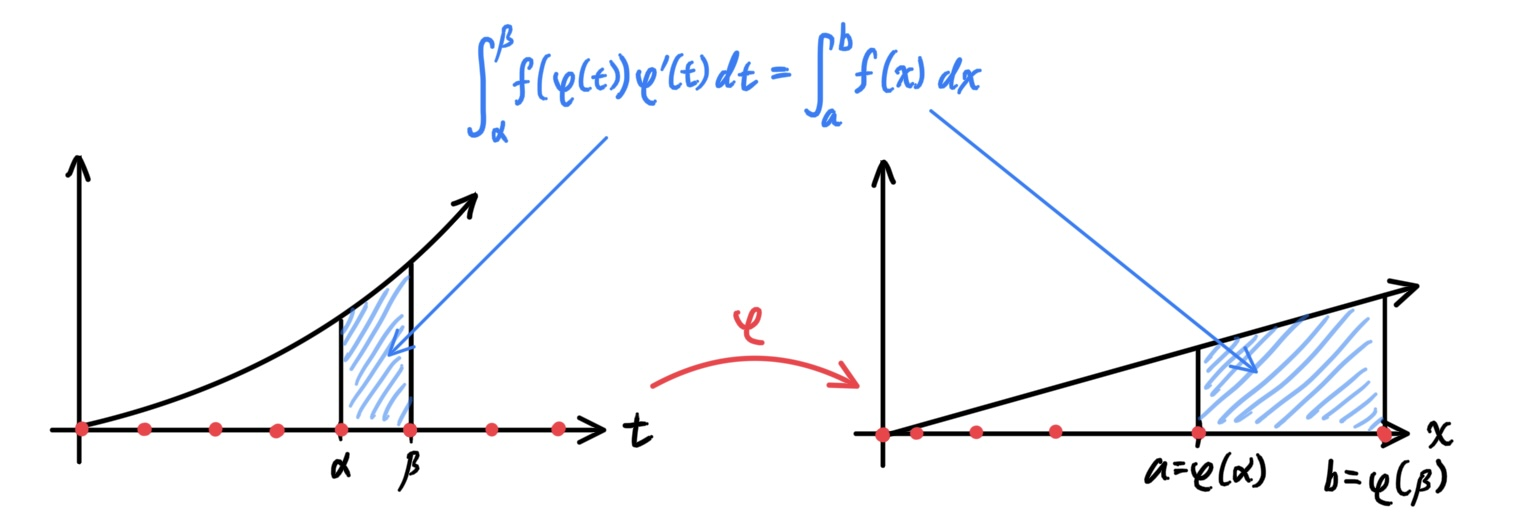
\includegraphics[scale=0.25]{img/Change_of_Variable_Analysis_Integral.jpg}
    \end{center}
    \end{theorem}
    \begin{proof}
    We prove a slightly weaker form of the theorem with the additional hypothesis that $\varphi$ is strictly monotonic. 
    \end{proof}

    \subsubsection{Additive Interval Functions and the Integral}
    In this section we take a step back and construct the integral in a more abstract sense, using the concepts of an additive interval function. 

    \begin{definition}[Additive Interval Function]
      An \textbf{additive (oriented) interval function} is a function 
      \[(\alpha, \beta) \mapsto I(\alpha, \beta) \in \mathbb{R}\]
      that assigns a number $I(\alpha, \beta)$ to each ordered pair of points $(\alpha, \beta)$ of a fixed closed interval $[a, b]$ in such a way that the following equality holds for any triple of points $\alpha, \beta, \gamma \in [a, b]$. 
      \[I(\alpha, \gamma) = I(\alpha, \beta) + I(\beta, \gamma)\]
      Notice that the integral holds this property, shown in the theorem on the symmetric property of the integral. It follows that all additive interval functions are anticommutative: 
      \[I(\alpha, \beta) + I(\beta, \alpha) = 0\]
      which immediately results in
      \[I(\alpha, \alpha) = 0\]
    \end{definition}

    \begin{lemma}[Generating Functions of Additive Interval Functions]
      For any function $x \mapsto \mathcal{F}(x)$ that maps points on the interval $[a, b]$ to $\mathbb{R}$, we set
      \[\mathcal{F}(x) \equiv I(a, x)\]
      and by additivity we have
      \[I(\alpha, \beta) = I(\alpha, \beta) - I(a, \alpha) = \mathcal{F}(\beta) - \mathcal{F}(\alpha)\]
      and thus, every additive oriented interval function has the form 
      \[I(\alpha, \beta) = \mathcal{F}(\beta) - \mathcal{F}(\alpha)\]
      By constructing $I$ in this manner, we say that \textbf{the function $\mathcal{F}$ generates the additive function $I$}. 
    \end{lemma}

    \begin{example}
    If $f \in \mathcal{R}[a, b]$, the function $\mathcal{F} = \int_a^x f(t)\,dt$ generates the additive function
    \[I(\alpha, \beta) = \mathcal{F}(\beta) - \mathcal{F}(\alpha) = \int_a^\beta f(t)\,dt - \int_a^\alpha f(t)\,dt = \int_\alpha^\beta f(t)\,dt\]
    \end{example}

    We conclude by stating a sufficient condition for an additive interval function to be generated by an integral. 
    \begin{theorem}
    Suppose the additive function $I(\alpha, \beta)$ defined for points $\alpha, \beta \in [a, b]$ has the property that, for some known function $f \in \mathcal{R}[a, b]$, 
    \[\inf_{x \in [\alpha, \beta]} f(x) (\beta - \alpha) \leq I(\alpha, \beta) \leq \sup_{x \in [\alpha, \beta]} f(x) (\beta - \alpha)\]
    holds for any closed interval $[\alpha, \beta] \subset [a, b]$ ($\alpha \leq \beta$). Then, the additive function $I$ must be the definite integral
    \[I(a, b) = \int_a^b f(x)\,dx\]
    \end{theorem}

    This theorem is extremely useful. It says that if we have any abstract additive interval function $I(\alpha, \beta)$ that satisfies the properties above, then it \textbf{must} be generated by an integral with variable upper limit, meaning that (by the previous example) $I$ itself must be a definite integral! 

    \subsubsection{Arc Length}
    When modeling systems in physics, one of the most fundamental tools we use are path functions that models the movement of a particle in $\mathbb{R}^3$. 

    \begin{definition}[Path]
      A \textbf{path} in $\mathbb{R}^3$ is a continuous mapping $r: [a, b] \subset \mathbb{R} \longrightarrow \mathbb{R}^3$ defined
      \[t \mapsto \big(x(t), y(t), z(t)\big)\]
      of an interval of the real line into $\mathbb{R}^3$ defined by the (continuous) scalar functions $x, y, z$. The endpoints 
      \[A = \big(x(a), y(a), z(a)\big) \text{ and } B = \big(x(b), y(b), z(b)\big)\]
      in $\mathbb{R}^3$ are called the \textbf{initial point} and \textbf{terminal point} of the path. Furthermore, a path is \textbf{closed} if its initial and terminal points coincide. 
    \end{definition}

    \begin{definition}[Support]
      If $\Gamma: I \longrightarrow \mathbb{R}^3$ is a path, the image $\Gamma(I) \subset \mathbb{R}^3$ is called the \textbf{support} of the path. 
    \end{definition}

    \begin{definition}[Simple Paths]
      A path $\Gamma: I \longrightarrow \mathbb{R}^3$ that is injective is called a \textbf{simple path}, or a \textbf{paramaterized curve}, and its support is called a \textbf{curve} in $\mathbb{R}^3$. 

      A closed path $\Gamma: [a, b] \longrightarrow \mathbb{R}^3$ is called a \textbf{simple closed path/curve} if the path $\Gamma: [a, b) \longrightarrow \mathbb{R}^3$ is simple. 
    \end{definition}

    \begin{definition}[Smooth Paths]
      A path $\Gamma: [a, b] \longrightarrow \mathbb{R}^3$ is $C^k$ smooth if the functions $x(t), y(t), z(t)$ are $C^k$ smooth. $\Gamma$ is \textbf{piecewise smooth} if the closed interval $[a, b]$ can be partitioned into a finite number of closed intervals on each of which the corresponding restriction of $\Gamma$ is smooth. 
    \end{definition}

    Now, we are ready to construct the length of a smooth path $\Gamma: [a, b] \longrightarrow \mathbb{R}^3$. Our initial ideas about the length $l[a, b]$ of the path traversed during the time interval $\alpha \leq t \leq \beta$ are as follows: 
    \begin{enumerate}
      \item If $\alpha < \beta < \gamma$, then $l$ is an additive interval function.
      \[l[\alpha, \gamma] = l[\alpha, \beta] + l[\beta, \gamma]\]
      \item If $v(t) = \big( x^\prime (t), y^\prime (t), z^\prime (t)\big)$ is the velocity of the point at time $t$, then 
      \[\int_{x \in [\alpha, \beta]} |v(t)| (\beta - \alpha) \leq l[\alpha, \beta] \leq \sup_{x \in [\alpha, \beta]} |v(t)| (\beta - \alpha)\]
    \end{enumerate}
    Thus, if the functions $x, y, z$ are continuously differentiable on $[a, b]$, this is sufficient condition (by the theorem in the previous subsection) that the additive function $l$ is an integral.

    \begin{definition}[Arc Length Integral]
      The length of a smooth path $\Gamma: [a, b] \longrightarrow \mathbb{R}^3$ is defined by 
      \[l[a, b] \equiv \int_a^b |\Gamma^\prime (t)|\,dt \equiv \int_a^b \sqrt{x^{\prime 2} (t) + y^{\prime 2} (t) + z^{\prime 2} (t)}\, dt\]
      We can visualize this by partitioning the interval $[a, b]$ into the intervals $\Delta_i$, each with point $\xi_i \in \Delta_i$. This would partition the path to $\Gamma(\Delta_i)$, each with points $\Gamma(\xi_i)$, and at each point $\Gamma(\xi_i)$, we can imagine the velocity vector of the curve. By taking the magnitude of this vector $\Gamma^\prime (\xi_i)$, we multiply it by the length of the interval $\Delta x_i$ to get one rectangle, creating an approximation for one partition of the path. 
      \begin{center}
          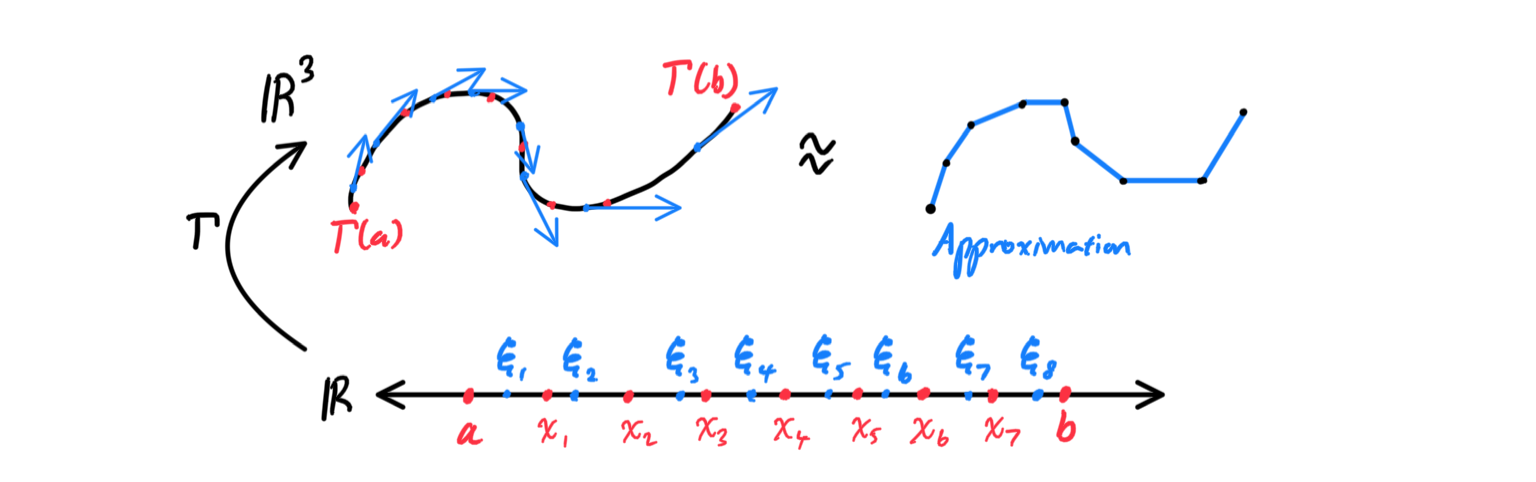
\includegraphics[scale=0.25]{img/Arc_Length_Integral.PNG}
      \end{center}
      An immediate result of this formula is the formula for the length of a graph of a function $f: [a, b] \longrightarrow \mathbb{R}$ in $\mathbb{R}^2$, by looking at the paramaterization $t \mapsto \Gamma(t) = \big(t, f(t)\big)$. 
      \[l[a,b] \equiv \int_a^b \sqrt{1 + (f^\prime (t))^2}\,dt\]
    \end{definition}

    The question on the effect of paramaterization on the integral now arises. 

    \begin{definition}[Admissible Change of Parameter]
      The path $\Tilde{\Gamma}: [\alpha, \beta] \longrightarrow \mathbb{R}^3$ is obtained from $\Gamma: [a, b] \longrightarrow \mathbb{R}^3$ by an \textbf{admissible change of parameter} if there exists a smooth mapping 
      \[T: [\alpha, \beta] \longrightarrow [a, b]\]
      such that $T(\alpha) = a, T(\beta) = b$, $T^\prime (\tau) > 0$ (that is, the reparamaterization $T$ is monotonic) on $[\alpha, \beta]$, and 
      \[\Tilde{\Gamma} = \Gamma \circ T\]
      The series of mappings can be represented with the following commutative diagram, where $I_{\alpha, \beta} = [\alpha, \beta] \subset \mathbb{R}$ and $I_{a, b} = [a, b] \subset \mathbb{R}$. 
      \[
        \begin{tikzcd}
          I_{\alpha, \beta} \arrow{r}{T} \arrow{rd}{\Tilde{\Gamma}}& I_{a, b} \arrow{d}{\Gamma}\\
           & \mathbb{R}^3
        \end{tikzcd}
      \]
      or with the more detailed visual below (Note that the points are labeled $0, 1, 2, 3, 4, 5$ do not represent numerical values, but rather the order in which the points are paramaterized. We can see from this ordering that $T$ is monotonic.)
      \begin{center}
          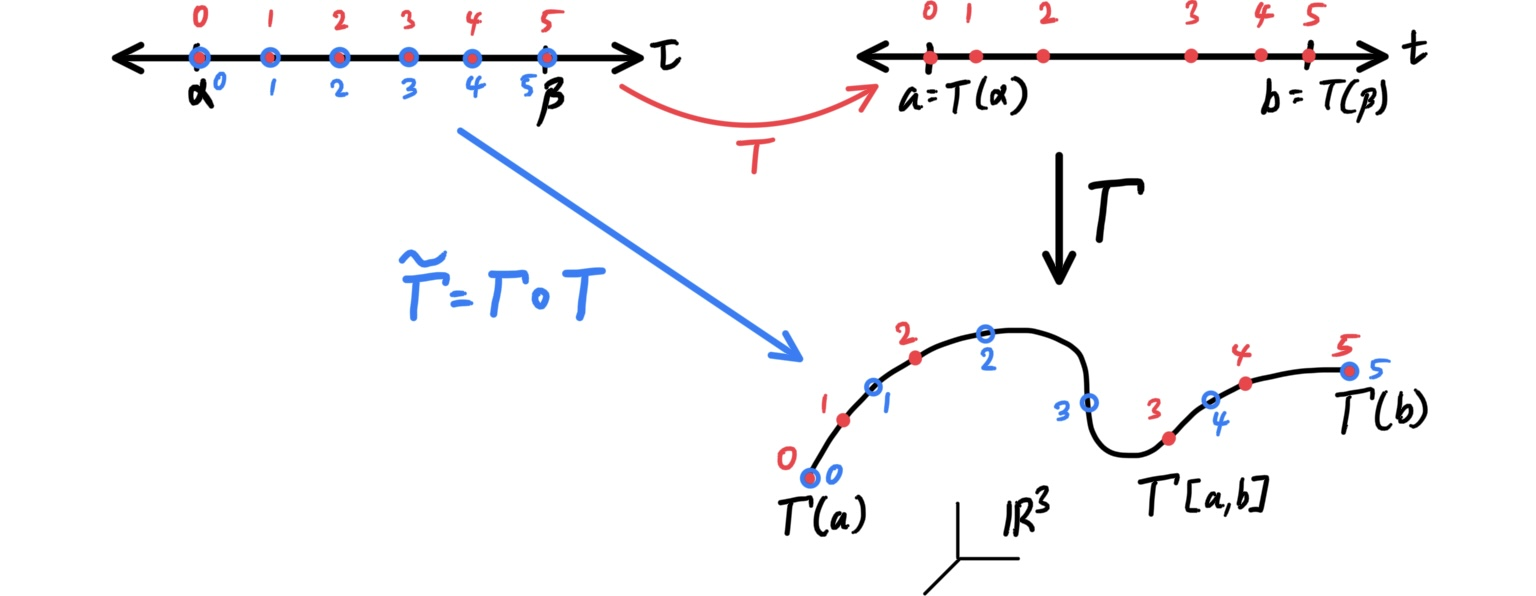
\includegraphics[scale=0.25]{img/Admissible_Change_of_Parameter.jpg}
      \end{center}
    \end{definition}

    \begin{theorem}[Invariance of Arclength Integral under Admissible Change of Parameters]
    If a smooth path $\Tilde{\Gamma}: [\alpha, \beta] \longrightarrow \mathbb{R}^3$ is obtained from a smooth path $\Gamma: [a, b] \longrightarrow \mathbb{R}^3$ by an admissible change of parameter, then the lengths of the two paths are equal. That is, a
    \[\int_a^b |\Gamma^\prime (t) |\,dt = \int_\alpha^\beta |\Tilde{\Gamma}^\prime (t)|\,dt \equiv \int_\alpha^\beta |(\Gamma \circ T)^\prime (t)|\,dt\]
    \end{theorem}

  \subsection{Improper Integrals}

    Due to some limitations of the Riemann integral, we cannot integrate over "singularities" where either the interval or the function is unbounded. We develop the tools of improper integration to deal with this problem; there are two types of improper integrals. 

    \begin{definition}[Improper Integral of Unbounded Interval]
      Suppose the function $x \mapsto f(x)$ is defined on the interval $[a, +\infty)$ and is integrable on every closed interval $[a, b]$ contained in that interval. Then, we call the following term
      \[\int_a^{+\infty} f(x)\,dx \equiv \lim_{b \rightarrow + \infty} \int_a^b f(x)\,dx\]
      the \textbf{improper Riemann integral of $f$ over the interval $[a, +\infty)$} and 
      \[\int_{-\infty}^b f(x)\,dx \equiv \lim_{a \rightarrow -\infty} \int_a^b f(x)\,dx \]
      the \textbf{improper Riemann integral of $f$ over the interval $(-\infty, b]$}.If the limit exists, then we say that the integral \textbf{converges} and \textbf{diverges} otherwise. 
    \end{definition}

    \begin{definition}[Improper Integral of Unbounded Function]
      Suppose the function $x \mapsto f(x)$ is defined on the interval $[a, B)$ and integrable on any closed interval $[a, b] \subset [a, B)$. Then, we call the following term
      \[\int_a^B f(x)\,dx \equiv \lim_{b \rightarrow B^-} \int_a^b f(x)\,dx\]
      the \textbf{improper Riemann integral of $f$ over interval $[a, B)$} and
      \[\int_A^b f(x)\,dx \equiv \lim_{a \rightarrow A^+} \int_a^b f(x)\,dx\]
      the \textbf{improper Riemann integral of $f$ over interval $(A,b]$}.
    \end{definition}

    For cohesiveness, we can combine these two definitions of improper integrals into the following one. 

    \begin{definition}[Improper Integrals]
      Let $[a, \omega)$ be a finite or infinite interval and $x \mapsto f(x)$ a function defined on that interval and integrable over every closed interval $[a, b] \subset [a, \omega)$. Then, by definition
      \[\int_a^\omega f(x)\,dx \equiv \lim_{b \rightarrow \omega} \int_a^b f(x)\,dx\]
      if this limit exists as $b \rightarrow \omega, b \in [a, \omega)$. Similarly, given the finite or infinite interval $(\omega, b]$ with $f$ integrable over every closed interval $[a, b] \subset (\omega, b]$, we have
      \[\int_\omega^b f(x)\,dx \equiv \lim_{a \rightarrow \omega} \int_a^b f(x)\,dx\]
      Note that if $\omega \in \mathbb{R}$ and $f \in \mathcal{R}[a, \omega]$, the improper integral is equivalent to the regular Riemann integral. 
      \[\int_a^\omega f(x) = \lim_{b\rightarrow \omega} \int_a^b f(x)\,dx\]
    \end{definition}

    \begin{lemma}[Properties of the Improper Integral]
      Suppose $f, g$ are functions defined on interval $[a, \omega)$ (without loss of generality, we let $\omega$ be the upper limit of integration) and integrable on every closed interval $[a, b] \subset [a, \omega)$. Suppose the improper integrals 
      \[\int_a^\omega f(x)\,dx \text{ and } \int_a^\omega g(x)\,dx\]
      are well-defined. 
      \begin{enumerate}
        \item For any $\lambda_1, \lambda_2 \in \mathbb{R}$ the function $(\lambda_1 f + \lambda_2 g)(x)$ is integrable in the improper sense on $[a, \omega)$ and
        \[\int_a^\omega (\lambda_1 f + \lambda_2 g)(x)\,dx = \lambda_1 \int_a^\omega f(x)\,dx + \lambda_2 \int_a^\omega g(x)\,dx\]
        \item For any $c \in [a, \omega)$, 
        \[\int_a^\omega f(x)\,dx = \int_a^c f(x)\,dx + \int_c^\omega f(x)\,dx\]
        \item If $\varphi: [\alpha, \gamma) \longrightarrow [a, \omega)$ is a smooth strictly monotonic mapping with $\varphi(\alpha) = a$ and $\varphi(\beta) \rightarrow \omega$ as $\beta \rightarrow \gamma^-$, then the improper integral of the function $t \mapsto (f \circ \varphi)(t) \varphi^\prime (t)$ over $[\alpha, \gamma)$ exists and 
        \[\int_a^\omega f(x)\,dx = \int_\alpha^\gamma (f \circ \varphi)(t) \varphi^\prime (t)\,dt\]
      \end{enumerate}
    \end{lemma}

    \subsubsection{Convergence of an Improper Integral}

      Note that by definition, an improper integral 
      \[\int_a^\omega f(x)\,dx \equiv \lim_{b \rightarrow \omega} \int_a^b f(x) \,dx\]
      is a limit of the function 
      \[\mathcal{F}(b) \equiv \int_a^b f(x)\,dx\]
      as $b \rightarrow \omega$. This means that we can use the Cauchy criterion to determine the convergence of this limit, and hence, existence of this improper integral. 

      \begin{theorem}[Cauchy Criterion for Convergence of an Improper Integral]
      If the function $x \mapsto f(x)$ is defined on the interval $[a, \omega)$ and integrable on every closed interval $[a, b] \subset [a, \omega)$, then the integral 
      \[\int_a^\omega f(x)\,dx\]
      converges if and only if for every $\epsilon > 0$ there exists $B \in [a, \omega)$ such that the relation
      \[\Bigg| \int_{b_1}^{b_2} f(x)\,dx \bigg| < \epsilon\]
      holds for any $b_1, b_2 \in [a, \omega)$ satisfying $B < b_1$ and $B < b_2$. 
      \end{theorem}
      \begin{proof}
      We have
      \[\int_{b_1}^{b_2} f(x)\,dx = \int_a^{b_2} f(x)\,dx - \int_a^{b_1} f(x)\,dx = \mathcal{F}(b_2) - \mathcal{F}(b_1)\]
      and therefore the condition is simply the Cauchy criterion for the existence of a limit for the function $\mathcal{F}(b)$ as $b \rightarrow \omega$. 
      \end{proof}

      \begin{definition}[Absolute Convergence of an Improper Integral]
        The improper integral 
        \[\int_a^\omega f(x)\,dx\]
        \textbf{converges absolutely} if the integral
        \[\int_a^\omega |f|(x)\,dx\]
        converges. Clearly, the inequality
        \[\Bigg| \int_{b_1}^{b_2} f(x)\,dx \Bigg| \leq \Bigg| \int_{b_1}^{b_2} |f|(x)\,dx \Bigg|\]
        implies that if an improper integral converges absolutely, then it converges. 
      \end{definition}

      This study of absolute convergence reduces to the study of convergence of integrals of nonnegative functions. The following lemma is useful in determining convergence of such functions. 

      \begin{lemma}
        Let there be a function $f$ defined on interval $[a, \omega)$ that is also integrable over every closed interval $[a, b] \subset [a, \omega)$. If $f(x) \geq 0$ on $[a, \omega)$, then the improper integral 
        \[\int_a^\omega f(x)\,dx\]
        exists if and only if the function 
        \[\mathcal{F}(b) \equiv \int_a^b f(x)\,dx\]
        is bounded on $[a, \omega)$. 
      \end{lemma}
      \begin{proof}
      It is clear that 
      \[\int_a^\omega f(x)\,dx = \lim_{b \rightarrow \omega} \mathcal{F}(b)\]
      If $f(x)\geq 0$, then the function $\mathcal{F}(b)$ is nondecreasing on $[a, \omega)$ and therefore has a limit as $b \rightarrow \omega$ only if it is bounded (since every monotonically increasing sequence that is bounded always converges). 
      \end{proof}

      This leads to the familiar integral test for convergence of a series. 

      \begin{theorem}[Integral Test for Convergence of a Series]
      If the function $x \mapsto f(x)$ is defined on the interval $[1, +\infty)$, nonnegative, nonincreasing, and integrable on each closed interval $[1, b] \subset [1, +\infty)$, then the series 
      \[\sum_{n=1}^\infty f(n) = f(1) + f(2) + \ldots\]
      and the integral 
      \[\int_a^{+\infty} f(x)\,dx\]
      either both converge or both diverge. 
      \end{theorem}

      We can use the comparison test analogue to determine convergence of improper integrals. 

      \begin{theorem}[Comparison Test for Convergence of Improper Integrals]
      Suppose the functions $f(x), g(x)$ are defined on the interval $[a, \omega)$ and integrable on any closed interval $[a, b] \subset [a, \omega)$. If 
      \[0 \leq f(x) \leq g(x)\]
      on $[a, \omega)$, then 
      \[\int_a^\omega g(x)\,dx \text{ converges} \implies \int_a^\omega f(x)\,dx \text{ converges}\]
      and the inequality 
      \[\int_a^\omega f(x)\,dx \leq \int_a^\omega g(x)\,dx\]
      holds. Also, 
      \[\int_a^\omega f(x)\,dx \text{ diverges} \implies \int_a^\omega g(x)\,dx \text{ diverges}\]
      \end{theorem}
    
    \subsubsection{Improper Integrals with Multiple Singularities}

      \begin{definition}[Improper Integral with Both Limits as Singularities]
        Given singularities $\omega_1, \omega_2$, the improper integral is defined
        \[\int_{\omega_1}^{\omega_2} f(x)\,dx \equiv \int_{\omega_1}^c f(x)\,dx + \int_c^{\omega_2} f(x)\,dx\]
        where $c$ is an arbitrary point in $(\omega_1, \omega_2)$. 
      \end{definition}

    \begin{example}[Gaussian Integral]
    The integral 
    \[\int_{-\infty}^{+\infty} e^{-x^2}\,dx = \sqrt{\pi}\]
    \end{example}



\end{document}

